\chapter*{怎么读这份批注稿}\label{ux600eux4e48ux8bfbux8fd9ux4efdux6279ux6ce8ux7a3f}
\addcontentsline{toc}{chapter}{怎么读这份批注稿}

这是\textbf{投稿前的审读稿}，针对 \texttt{paper/*.md}（TALG Empirical
Track 目标稿）。正文一字未改；
左栏是原文，右栏是批注卡片，被批注的句子在原文里带底色并跟一个上标编号。

所有批注在 \texttt{paper/*.md} 里都是 HTML
注释，\texttt{latex/build\_paper.sh} 会原样剥掉， 因此
\texttt{talg\_main.pdf} 不受影响（构建后已核验：正文中批注关键词出现 0
次）。

\section*{七个审读视角}\label{ux4e03ux4e2aux5ba1ux8bfbux89c6ux89d2}
\addcontentsline{toc}{section}{七个审读视角}

学位论文那套角色按投稿场景重新配了权：读者不再是二审考官和答辩老师，而是审稿人。

\begin{itemize}
\tightlist
\item
  \textbf{P1 领域外审稿人} ------
  做算法但不做在线匹配。管：常数与记号有没有出处、定义是否自足。
\item
  \textbf{P2 领域审稿人} ------
  真正对口的那位，\textbf{权重最高}。管：断言强度与证据是否匹配、
  定理的条件有没有被摘要吞掉、量化结论能不能复核。
\item
  \textbf{P3 英语文字编辑} ------ 长句、冗词、摘要长度、表述歧义。
\item
  \textbf{P4 体例校对} ------
  符号一致、交叉引用、占位符、正文与表格数字一致、venue 体例。
\item
  \textbf{P5 审稿意见预演} ------ 这句话会招来哪一条 reviewer
  comment，rebuttal 时能不能接住。
\item
  \textbf{P6 初次读者} ------ 摘要与贡献列表能否在一页内让人决定继续读。
\item
  \textbf{P7 复现审稿人}（新增）------ artifact evaluation
  视角：审稿人照着跑，会在哪一步卡住。
  确定性、外部数据、脚本引用都归它管。
\end{itemize}

\section*{严重度}\label{ux4e25ux91cdux5ea6}
\addcontentsline{toc}{section}{严重度}

\begin{itemize}
\tightlist
\item
  \textbf{必改}（红）------
  会被审稿人直接写进意见，或存在事实/一致性风险。
\item
  \textbf{建议}（橙）------ 明显影响可读性或说服力。
\item
  \textbf{可选}（蓝）------ 风格偏好。
\end{itemize}

逐条清单见 \texttt{paper/review/*.review.md}。

\clearpage

\chapter{The Limits of Predictions for Online Bipartite Matching: A
Unified Experimental Study and a Budget--Stakes
Law}\label{the-limits-of-predictions-for-online-bipartite-matching-a-unified-experimental-study-and-a-budgetstakes-law}

\section{Abstract}\label{abstract}

\revpair{Learning-augmented (``with-predictions'') algorithms for online
bipartite matching have proliferated: MinPredictedDegree consumes a
per-node degree predictor, and a family of \emph{test-and-fallback}
schemes tests a type-histogram prediction on a sublinear prefix of the
arrivals before committing to follow it or to fall back on an
advice-free baseline. These algorithms have been analyzed in isolation
--- on different input models, against different error models, and
largely in theory. \revhl{revShould}{We give the first unified experimental study}\revhlid{revShould}{0-05}, placing
all of them on a single harness with a common structured
prediction-error model, a common optimum, and confidence intervals,
across synthetic graphs, six real-world graphs, and real request traces.
Our central finding is that, on average-case (known-i.i.d.) inputs, the
value of predictions is \textbf{robustness insurance, not a performance
lever}: the advice-free baseline is already near-optimal, so the
\emph{consistency} upside of good advice is small, whereas unguarded
prediction-following can crash far below the baseline --- and the
practical worth of the sophisticated algorithms is precisely that they
never do. We then prove what the wall \emph{costs}. \revhl{revMust}{For the
test-and-fallback class we establish a sharp, two-sided}\revhlid{revMust}{0-01}\textbf{budget--stakes law}: deciding whether to follow the advice
requires --- and, via an explicit one-line rule, only requires --- a
prefix of length \(\tilde\Theta(\sigma^2/g^2)\): the instance's
specialist mass \(\sigma^2\) (exactly twice its baseline slack) \revhl{revShould}{divided
by the squared stakes}\revhlid{revShould}{0-04} \(g\) (what good advice gains over the baseline),
\revhl{revMust}{independent of the instance length}\revhlid{revMust}{0-02}. The lower half binds \emph{every}
decision rule; the upper half refutes the natural conjecture that the
hardness of tolerant distribution testing blocks all sublinear rules ---
the decision-relevant statistic is the \emph{payoff} of following, which
is exponentially cheaper to test than the prediction's distance --- a
prescription we validate on the benchmark, where a constant-free
payoff-testing rule avoids the threshold pathologies of the deployed
tests. Because the stakes are capped by the baseline slack, on
strong-baseline instances the price exceeds the horizon: upsides below
\(\approx\sqrt{(1-\rho_{\mathrm{base}})/n}\) are uncapturable by any
rule at any prefix length, and the upsides we measure sit in that range.
Experiments and theory deliver one message: \textbf{on average-case
matching, the advice's upside is smaller than the price of finding out
whether to trust it.}}{\revcard{revMust}{0-01 · P2 领域审稿人 · 必改 · sharpness 无条件陈述}{%
\textbf{问题}\hspace{0.4em}摘要与引言都把这条律说成 sharp、two-sided、无条件。但 §7.5 的两侧只有在「赌注由常数比例的 specialist mass 以可比信号承载」（Cauchy–Schwarz 那步）时才相接，而 §7.8 自己承认在低信号 sliver 上两侧可以差 sigma\textasciicircum{}2*eps\_W/g 倍，且该情形开放。审稿人对照 §7.8 读摘要，会直接写 the claimed sharpness is conditional and the condition is not stated up front。\par
\textbf{建议}\hspace{0.4em}摘要与引言各加一个限定从句：sharp up to logarithms whenever the stakes are carried by a constant fraction of the specialist mass（并指向 §7.8 的开放情形）。宁可摘要保守，§7 再给完整版。}
\revcard{revMust}{0-02 · P4 体例校对 · 必改 · 赌注符号三套}{%
\textbf{问题}\hspace{0.4em}同一个量在摘要与引言里有三个名字：g（stakes）、delta（引言末尾的 stakes cap）、以及 §7.5(ii) 的 delta/Delta（gain/loss）。审稿人读到 delta <= 2 eps (1-rho) 时会以为它和 g 是两个量。\par
\textbf{建议}\hspace{0.4em}全文统一：g = 赌注（scenario pair 的 payoff gap），delta/Delta 只在 Lemma 1 的 gain/loss 语境里出现，并在首次出现处写明二者关系。引言那句 cap 改用 g。}}

\revpair{\mbox{}}{\revcard{revShould}{0-03 · P3 英语文字编辑 · 建议 · 摘要过长}{%
\textbf{原文}\hspace{0.4em}\textquotedblleft (摘要整体)\textquotedblright\par
\textbf{问题}\hspace{0.4em}摘要约 430 词、单段、含四个带公式的从句。ACM/TALG 的摘要通常 200–250 词，且审稿人先读它决定要不要认真读。\par
\textbf{建议}\hspace{0.4em}压到 250 词以内：前三句给问题与实验发现，中间两句给律与它买到什么，最后一句金句。公式只留 sigma\textasciicircum{}2/g\textasciicircum{}2 一个。}
\revcard{revShould}{0-04 · P3 英语文字编辑 · 建议 · 表述歧义}{%
\textbf{问题}\hspace{0.4em}读作「被平方后的赌注 g 除」，但公式是 sigma\textasciicircum{}2/g\textasciicircum{}2，应是」除以赌注 g 的平方」。\par
\textbf{建议}\hspace{0.4em}改成 divided by the square of the stakes \$g\$。}}

\revpair{\mbox{}}{\revcard{revShould}{0-05 · P5 审稿意见预演 · 建议 · novelty 断言的可核查性}{%
\textbf{问题}\hspace{0.4em}两处 first/new 都是可被单条反例推翻的断言，而支撑它们的检索范围只在 §7 与 §9 零散提及。这是单作者投稿最容易被要求补充的地方。\par
\textbf{建议}\hspace{0.4em}在 §9 开头加一句可核对的范围声明（检索了哪些库与会议、关键词、截止时间），并让摘要与 §7 的 new 都指向它。}
\revcard{revShould}{0-06 · P6 初次读者 · 建议 · 贡献列表过长}{%
\textbf{原文}\hspace{0.4em}\textquotedblleft (C1)-(C5) 五条贡献\textquotedblright\par
\textbf{问题}\hspace{0.4em}五条贡献占了近一页，C4 与 C5 各自内部又套了三到四个子项。审稿人常常只看这一页就形成初判。\par
\textbf{建议}\hspace{0.4em}每条压到两到三行：一句说贡献是什么，一句说它在哪一节。C4 的实现细节（Jensen 偏差、bootstrap）移到 §5.4。}}

\revpair{\begin{center}\rule{0.5\linewidth}{0.5pt}\end{center}}{}

\section{1. Introduction}\label{introduction}

\revpair{Online bipartite matching is the canonical model of irrevocable
sequential allocation: offline resources are known in advance, requests
arrive one at a time, and each request must be matched to an available
neighbor --- or dropped --- immediately and irrevocably, before the rest
of the input is seen. It underlies ad allocation, ride-hailing dispatch,
organ exchange, and request routing in serving systems. Classical online
algorithms --- Greedy, KVV Ranking {[}KVV90{]}, and the
stochastic-matching algorithms of Feldman et al. {[}FMMM09{]} and
Jaillet--Lu {[}JL14{]} --- are analyzed through the worst-case
competitive ratio.}{}

\revpair{A now-large body of work augments these algorithms with a
\emph{prediction} about the input and asks for two guarantees at once:
\textbf{consistency} (near-optimal performance when the prediction is
good) and \textbf{robustness} (no worse than an advice-free baseline
when the prediction is arbitrarily bad) {[}LV18, WZ20{]}. For online
matching specifically, two strands have emerged. MinPredictedDegree
(MPD) {[}ACI22{]} matches each arrival to its available neighbor of
minimum \emph{predicted} degree, protecting scarce resources; it is
robust by construction (a useless predictor reduces it to Ranking). A
second strand --- the \emph{test-and-fallback} algorithms of Choo et
al.~{[}Choo24{]} and Burathep--Erlebach--Moses {[}BEM26{]} --- is
explicitly adaptive: it Mimics a type-histogram prediction on a
sublinear prefix of arrivals, tests whether the observed arrivals match
the prediction, and then either continues to follow it or falls back to
Ranking.}{}

\revpair{These algorithms have been studied \emph{in isolation} --- each on its
own input family, against its own error model, and largely through
worst-case theory. As a result, three basic questions have no empirical
answer. How do the algorithms actually compare, head to head, under one
prediction-error model? How much does a prediction help, and at what
cost, on realistic inputs? And --- most importantly --- \emph{why} does
the practical experience with these algorithms feel so different from
their worst-case promise? This paper answers all three, with a unified
experimental study and a theorem that explains what the study finds.}{}

\revpair{\textbf{A unified experimental study.} We place the advice-free
baselines, the MPD family (and its Feldman/Jaillet--Lu augmentations),
and the test-and-fallback algorithms on a single harness: common graph
families, a common structured prediction-error model, a common optimum
computed by Hopcroft--Karp, and 95\% confidence intervals throughout. We
also port the blind-follow-with-switching \emph{combiner} of Chłędowski
et al.~{[}Chl21{]} --- the ``cheap worst-case insurance'' from the
caching literature --- and benchmark it (we do not claim it as new). The
study runs across synthetic graphs spanning the difficulty range, six
real-world graphs from the Network Repository, and real request traces.}{}

\revpair{\textbf{The empirical wall.} Across every setting we observe the same
phenomenon, which we state as the paper's organizing thesis: \emph{on
average-case inputs the value of predictions is robustness insurance,
not a performance lever.} Concretely (Section 3): the advice-free
Ranking is already within a percent or two of the optimum, so the
consistency upside of even perfect advice is small; unguarded
prediction-following (blind Mimic, or MPD under adversarial predictions)
crashes \emph{below} the advice-free floor; and the entire practical
value of the sophisticated algorithms is that they refuse to crash. Two
distinct mechanisms deliver this --- the structural robustness of the
MPD-augmentations and the adaptive robustness of test-and-fallback ---
with different consistency/robustness trade-offs. We confirm the wall on
the six real graphs and on real traces, where a cheap, non-ML historical
predictor captures a meaningful fraction of the (small) oracle gap while
never dropping below the baseline (Section 6). We also report a negative
result: because MPD depends on its predictor only through the induced
\emph{order}, one might train the predictor with an order-aware loss
instead of regression, but on realistic features the two coincide ---
reinforcing that the predictor, once order-faithful, is not the
bottleneck.}{}

\revpair{\textbf{Why the wall is necessary --- and what it costs.} The empirical
wall is not an artifact of a particular generator or algorithm; it has a
price tag. Our main theoretical contribution (Section 7) is a two-sided
\textbf{budget--stakes law} for the test-and-fallback class. Informally:}{}

\revpair{\begin{quote}
Deciding whether to follow the advice costs a prefix of length
\(k^* = \tilde\Theta(\sigma^2/g^2)\), where \(g\) is the stakes (what
good advice gains over the baseline) and \(\sigma^2\), the arrival mass
on contested resources, equals exactly twice the baseline slack. Below
\(k^*\), \emph{no} decision rule is simultaneously consistent and
robust; at \(k^*\), an explicit one-line rule is.
\end{quote}}{}

\revpair{The lower half is information-theoretic --- it binds \emph{any}
measurable rule on the prefix, not merely the empirical-distance
threshold used in practice --- via a master consistency/robustness
inequality and a Hellinger computation. The upper half is a
\textbf{directional test}: classify each prefix arrival as agreeing or
disagreeing with the advice's local prediction, and follow iff
agreements win --- a rule we also implement, calibrate, and evaluate
head-to-head on the benchmark (§5.4). Its analysis rests on a
\emph{payoff identity} --- on the hard family, the advantage of
following is exactly half the mean of a per-sample observable --- which
also refutes the tempting stronger conjecture (and an earlier version of
our own claim) that tolerant-testing hardness {[}CJKL22{]} makes the
decision impossible for every sublinear rule: the advice's
\emph{distance} to the truth is indeed hard to test, and the field's
empirical-\(\ell_1\) thresholds are provably blind at sublinear
prefixes, but the decision-relevant \emph{payoff} is not. The wall then
re-emerges exactly where the experiments live: stakes are capped by the
baseline slack (\(\delta \le 2\varepsilon(1-\rho_{\mathrm{base}})\)), so
on strong-baseline instances the budget \(k^*\) exceeds the horizon
itself --- every upside below
\(\Theta(\sqrt{(1-\rho_{\mathrm{base}})/n})\) is uncapturable at
\emph{any} feasible prefix, and the upsides measured in Sections 3--6
sit in that range.}{}

\revpair{\textbf{Contributions.} - \textbf{(C1) The first unified benchmark} of
learning-augmented online-matching algorithms --- advice-free baselines,
the MPD family, and the test-and-fallback schemes --- on one harness
with a common error model, a common optimum, and confidence intervals
(Section 3). - \textbf{(C2) The robustness-insurance characterization.}
Unguarded followers crash below the advice-free floor; two mechanisms
(structural and adaptive) restore safety with distinct trade-offs; the
consistency upside is small on average-case inputs, so the value is
downside protection. Validated on synthetic graphs, six real graphs, and
real traces (Sections 3, 6). - \textbf{(C3) An empirical engagement with
the order-error theory.} MPD's loss is governed by a Kendall-τ order
error onto which several error models collapse; we characterize the
tightness and saturation of the known \(n{-}\mathrm{LIS}\) bound
{[}ACI22, App. D{]} rather than re-deriving order-dependence (Section
4). - \textbf{(C4) The first empirical study of test-and-fallback},
including a threshold-calibration pathology (a more accurate test can
make a worse decision), its recalibration and resolution limit, a
\textbf{constant-free payoff-testing rule} that avoids both threshold
pathologies --- its misjudgement \emph{falls} with prefix size exactly
where the thresholds' \emph{rises} --- and a benchmark of the dynamic
combiner exhibiting an irrevocability penalty that explains why matching
needs \emph{test-then-commit} (Section 5). - \textbf{(C5) The
budget--stakes law.} A sharp two-sided law for test-and-fallback: the
follow/fallback decision costs a prefix of
\(\tilde\Theta(\sigma^2/g^2)\) (baseline slack over squared stakes) for
\emph{any} rule (lower bound), and an explicit directional test achieves
it (upper bound). A payoff identity separates cheap payoff-testing from
provably hard distance-testing --- refuting, and reporting honestly, the
natural tolerant-testing impossibility --- and the corollary quantifies
the wall: on strong-baseline instances, upsides below
\(\Theta(\sqrt{(1-\rho_{\mathrm{base}})/n})\) are uncapturable at any
prefix length (Section 7).}{}

\revpair{The experiments and the law are two views of one fact. The experiments
discover a wall --- predictions buy insurance, not performance; the law
prices the wall --- verifying advice costs the inverse square of its
stakes, and average-case stakes cannot cover the bill. We adopt an
AI-inference serving instantiation as a running application case study
(Section 8) rather than a novelty claim, and we are careful throughout
to credit the prior results our findings build on and to state the scope
of each claim.}{}

\chapter{2. Setup}\label{setup}

\section{2.1 Model}\label{model}

\revpair{We work in the \textbf{known-i.i.d.} model of online bipartite matching.
There is a set \(R\) of \(n\) \textbf{offline resources} and a
\textbf{type graph} on \(r\) \textbf{online types}, where type \(\ell\)
has a neighborhood \(N(\ell)\subseteq R\) (the resources able to serve
it). An \textbf{instance} is generated by drawing \(m\) arrivals i.i.d.
from a distribution \(p\) over the \(r\) types; the \(i\)-th arrival
reveals its type (hence its neighborhood) and must be matched,
immediately and irrevocably, to a currently unmatched resource in its
neighborhood, or left unmatched. The type graph and \(p\) are known to
the algorithm; the realized arrival sequence is not. The classical
setting is \(r=n\) and \(m=n\) (each offline vertex a distinct type); we
also use \emph{few-types} instances (\(r\ll n\)), where a prefix
distribution-test is statistically meaningful.}{}

\revpair{We measure the \textbf{competitive ratio}
\(\rho(\mathrm{ALG}) = \mathbb{E}[|\mathrm{ALG}|] /
\mathbb{E}[|\mathrm{OPT}|]\), where \(\mathrm{OPT}\) is a maximum
matching of the \emph{realized} instance, computed exactly by
Hopcroft--Karp {[}HK73{]}. All reported ratios are Monte-Carlo estimates
with 95\% confidence intervals (Section 2.5). The advice-free baseline
we compare against throughout is KVV Ranking {[}KVV90{]}, whose ratio we
denote \(\rho_{\mathrm{base}}\) and call the \textbf{baseline strength}.}{}

\section{2.2 Algorithms}\label{algorithms}

\revpair{All the greedy-type algorithms share one primitive. Given a rank (a
total order) on the resources, \textbf{GreedyWithPermutation} matches
each arrival to its available neighbor of \emph{minimum rank}. The
advice-free baselines are three instances of this primitive together
with the two stochastic-matching algorithms:}{}

\revpair{\begin{itemize}
\tightlist
\item
  \textbf{SimpleGreedy} --- GreedyWithPermutation under the identity
  rank.
\item
  \textbf{Ranking} {[}KVV90{]} --- GreedyWithPermutation under a
  uniformly random rank; the baseline.
\item
  \textbf{Feldman} {[}FMMM09{]} and \textbf{Jaillet--Lu} {[}JL14{]} ---
  the known-i.i.d. stochastic-matching algorithms (a max-flow blue/red
  decomposition, and a cap-3 LP realized by max-flow with per-type list
  distributions, respectively).
\end{itemize}}{}

\revpair{\textbf{Degree predictions (object A).} MinPredictedDegree (MPD)
{[}ACI22{]} is GreedyWithPermutation ranked by ascending \emph{predicted
degree} \(\mu\in\mathbb{R}^{R}\): it matches to the available neighbor
predicted to be rarest. With \(\mu\) constant it reduces to Ranking;
with \(\mu\) the true realized degrees it is the consistency ceiling
(MinDegree). Following ACI, we also form the \textbf{augmentations}
Feldman(MPD) and JailletLu(MPD), which use the MPD rank only as the
tie-break of the greedy fallback, so the worst-case-optimal base
matching carries the load.}{}

\revpair{\textbf{Type-histogram advice (object B) and test-and-fallback.} The
advice is a count vector \(\hat c\in\mathbb{Z}_{\ge 0}^{r}\) over types
(equivalently a distribution \(q=\hat c/\|\hat
c\|_1\)). From \(\hat c\) we build an \emph{advice graph}
(\(\hat c_\ell\) copies of type \(\ell\)), compute a maximum matching
\(\hat M\) on it, and record, per type, the resources \(\hat M\) uses.
\textbf{FollowPrediction} (blind Mimic) routes every arrival according
to \(\hat M\). \textbf{TestAndMatch} {[}Choo24, BEM26{]} instead Mimics
a sublinear prefix of \(k\) arrivals, estimates the \(\ell_1\) distance
between the prefix type distribution and \(q\), and --- if the estimate
is at most a threshold \(\tau\) --- continues to Mimic, else falls back
to Ranking. The two variants differ only in an early-exit rule and in
\(\tau\) (Choo: \(\tau =
2(\hat n/n - \beta)\); BEM: \(\tau = 2(\hat n/n)(1-\beta)/(1+\beta)\)),
where \(\beta\) is the worst-case baseline ratio. Faithfulness note: the
papers' \(\ell_1\) tester {[}JHW18{]} has no deployable implementation
and the authors themselves fall back to an empirical-\(\ell_1\)
proof-of-concept; we do the same, and mark it as such.}{}

\revpair{\textbf{The combiner (a benchmarked baseline, not a contribution).} We
port the blind-follow-with-switching combiner of Chłędowski et
al.~{[}Chl21{]} --- run FollowPrediction and Ranking as shadow experts
and follow the leader with hysteresis --- to contextualize
test-and-fallback. We benchmark it; we do not claim it.}{}

\section{2.3 Prediction objects and the structured error
model}\label{prediction-objects-and-the-structured-error-model}

\revpair{To compare algorithms that consume \emph{different} prediction objects
(degree vectors \(\mu\) vs type histograms \(\hat c\)), we corrupt each
object with a per-family knob and report the families in parallel; this
heterogeneity is intrinsic and is precisely why no unified benchmark
existed.}{}

\revpair{For \textbf{degree predictions} we perturb the true degrees
\(\mu^\star\) with four structured error models, each returning both an
\(\ell_1\) \emph{magnitude} and a normalized \textbf{Kendall-\(\tau\)
order error} in \([0,1]\): \emph{random-flip} (replace a fraction of
entries by uniform noise), \emph{systematic-bias} (a monotone rescale
--- order-preserving, hence Kendall-\(\tau\equiv 0\) by construction),
\emph{adversarial} (reflect a fraction of entries, the most
order-damaging), and \emph{distribution-drift} (blend toward degrees
from an independently drawn graph of the same family). Because MPD
depends on \(\mu\) \emph{only through the induced order}, the
order/magnitude distinction is not cosmetic --- it is the axis Section 4
is about.}{}

\revpair{For \textbf{type-histogram advice} we perturb the realized counts
\(c^\star\) toward a concentrated (spiky) random target by a fraction
\(\eta\in[0,1]\) (\(\eta=0\): perfect advice, \(\hat c=c^\star\);
\(\eta=1\): advice unrelated to the truth), reporting the induced
\(\ell_1(p,q)\) as the advice-error axis for the test-and-fallback
experiments.}{}

\section{2.4 Consistency and
robustness}\label{consistency-and-robustness}

\revpair{For a prediction-consuming algorithm we call \(\rho\) under
\emph{perfect} advice its \textbf{consistency} and its worst-case
\(\rho\) over \emph{adversarial} advice its \textbf{robustness}. A
prediction algorithm is useful only if it is consistent \emph{and} never
falls (much) below \(\rho_{\mathrm{base}}\); the tension between the
two, and its fundamental limits for the test-and-fallback class, are the
subject of Sections 5 and 7.}{}

\section{2.5 Experimental methodology and
reproducibility}\label{experimental-methodology-and-reproducibility}

\revpair{The harness is a small dependency-light Python codebase
(NumPy/SciPy/NetworkX). We draw all randomness from independent,
reproducible streams via NumPy's spawn-based generators, and use
\textbf{paired trials}: within a comparison, every algorithm and every
error level reuses the same graph, arrival sequence, \(\mathrm{OPT}\),
and tie-break seed, so differences are attributable to the prediction
alone. Confidence intervals are 95\% normal-approximation half-widths
over trials. The Phase-2 portion reproduces a subset of Borodin,
Karavasilis \& Pankratov {[}Bor18{]}; \revhl{revShould}{every figure and table in this
paper is regenerated from a fixed seed by a single script}\revhlid{revShould}{1-02}, \revhl{revMust}{listed with
its output in Appendix}\revhlid{revMust}{1-01}{[}REPRO{]}.}{\revcard{revMust}{1-01 · P7 复现审稿人 · 必改 · 未解析的交叉引用}{%
\textbf{问题}\hspace{0.4em}这是一个没被替换掉的占位符，它已经原样印进 talg\_main.pdf 的正文（第 3 页）。而且论文里并没有复现附录——学位论文有，这篇没有。审稿人看到 Appendix [REPRO] 会立刻怀疑稿件的成熟度。\par
\textbf{建议}\hspace{0.4em}两件事：把占位符换成真正的指向；并补一个简短的复现附录（图表→脚本映射、种子、外部数据获取方式）。学位论文附录 A 可以直接压缩移植。}
\revcard{revShould}{1-02 · P7 复现审稿人 · 建议 · 外部数据前提}{%
\textbf{问题}\hspace{0.4em}第 6、8 节的真实图与 trace 结果需要先获取外部数据，而这句话让审稿人以为克隆代码即可复现全部。artifact evaluation 会当场卡住。\par
\textbf{建议}\hspace{0.4em}补半句区分自足脚本与需要外部数据的脚本，并给出后者的获取方式（与新增的复现附录合并）。}}

\revpair{One implementation detail is load-bearing for that claim. Three
preprocessing steps --- Feldman's and Jaillet--Lu's suggested matchings,
and the serving advice \(b\)-matching --- take a maximum flow and
consume its \emph{decomposition}, which, unlike the flow value, is not
unique; the solver picks one by iterating node containers. We therefore
label those networks' nodes with integers rather than strings, since
Python randomises string hashes per process and string labels made the
chosen decomposition, and every number derived from it, differ between
runs of the same script.}{}

\chapter{3. The Unified Benchmark}\label{the-unified-benchmark}

\revpair{This section places all three algorithm families on one harness and
establishes the paper's organizing thesis. We report competitive ratios
(mean \(\pm\) 95\% CI) as a function of prediction quality, in three
panels chosen to span the regimes each family was designed for.}{}

\section{3.1 Design}\label{design}

\revpair{The families consume different prediction objects, so each is driven by
its own corruption knob and reported in a parallel panel (Section 2.3);
the shared harness --- graphs, \(\mathrm{OPT}\), CI methodology, and the
advice-free floor --- is what makes the panels comparable.}{}

\revpair{\textbf{Instance format and notation.} Every panel uses the instance
format of Section 2.1: \(n\) offline resources, \(r\) online request
types, and \(m\) arrivals drawn i.i.d. from the type distribution;
throughout this section \(m=n\), so requests and resources are balanced.
The panels differ \emph{only} in the type graph connecting requests to
resources --- that single change is what moves the input between the
regimes the two prediction families were designed for. The three are
chosen so that a \emph{degree} predictor has strong signal, weak signal,
and no role at all, respectively:}{}

\revpair{\begin{itemize}
\tightlist
\item
  \textbf{Panel A --- heavy-tailed degrees (Zipf)} (\(n=1000\), 60
  trials): \revhl{revMust}{resource degrees follow a Zipf power law}\revhlid{revMust}{2-01} with exponent
  \(1.0\) --- a few resources are heavily contended while most are
  rarely eligible. This heavy-tailed profile gives a \emph{degree}
  predictor genuine signal to carry.
\item
  \textbf{Panel B --- left-regular \(d{=}5\)} (\(n=1000\), 60 trials):
  each arriving request connects to exactly \(d=5\) uniformly random
  resources, so resource degrees are nearly homogeneous --- the hard
  case for this family, where a degree predictor has almost no signal
  left to carry.
\item
  \textbf{Panel C --- few-types \(r{=}8\)} (\(n=2000\), 50 trials): only
  \(r=8\) distinct request types, each arriving \(\approx n/r=250\)
  times on average --- the near-perfect-matchable, few-types regime the
  \emph{histogram}-advice algorithms are calibrated for; their
  test-and-fallback test inspects a prefix of \(k=200\) arrivals.
\end{itemize}}{}

\revpair{Panels A and B thus exercise the degree-prediction family (MPD and its
augmentations); Panel C exercises the histogram-advice family
(FollowPrediction, TestAndMatch, and the combiner).}{}

\revpair{\textbf{Shared methodology.} Paired trials, independent random streams
and confidence intervals are exactly as in Section 2.5; the
panel-specific parameters are the ones listed above, and the intervals
are tight throughout (\(\pm0.001\)--\(0.003\)). The quality columns
instantiate the error models of Section 2.3 --- degree panels:
\emph{perfect} (true realized degrees), \emph{noisy} (random-flip at
strength \(\tfrac12\)), \emph{adversarial} (order-reversing reflection),
\emph{garbage} (independent random \(\mu\), \(\equiv\) Ranking); advice
panel: the true histogram blended toward a concentrated random target by
\(\eta\in\{0,0.3,0.6,1.0\}\) (\emph{perfect / mild / bad / garbage}).
The two sets of columns are \emph{not} commensurable --- they corrupt
different prediction objects with different knobs --- so only
within-panel comparisons carry meaning. \textbf{Table 1} presents each
panel's ratios beside its bar chart; the findings follow in Section 3.2.}{\revcard{revMust}{2-01 · P4 体例校对 · 必改 · 代码名进正文}{%
\textbf{问题}\hspace{0.4em}clvb\_zipf 是生成器标识符，带下划线出现在表里。审稿人不知道 clvb 是什么，也看不出这个面板测的是什么。\par
\textbf{建议}\hspace{0.4em}改成可读名（heavy-tailed degrees (Zipf)），把脚本标识符放进复现附录。}
\revcard{revMust}{2-02 · P4 体例校对 · 必改 · 三个 floor 不可比}{%
\textbf{原文}\hspace{0.4em}\textquotedblleft Ranking (floor) 0.948 / Greedy = Ranking (floor) 0.890 / Ranking (floor) 0.990\textquotedblright\par
\textbf{问题}\hspace{0.4em}三个面板的 floor 是三个不同的数，来自不同图族，表里没有任何提示；两族的质量列语义也不同却同名并排。审稿人第一反应是横向比较。\par
\textbf{建议}\hspace{0.4em}表注加一句：floor 是 Ranking 在该面板自身图族上的比值，面板之间不可比；两族的质量列同样只在面板内部可比。}}

\begin{table}[H]
\caption{The unified benchmark. Each panel's competitive ratios (means over paired
trials; every 95\% CI $\le 0.003$) sit beside their bar chart (error bars: 95\% CIs;
dashed line: advice-free floor; dotted: oracle ceiling). Bold marks the worst column of
each unguarded prediction-follower; all three fall below their own panel's floor. That
floor is instance-dependent --- it is Ranking's ratio on that panel's graph family, not a
constant --- so the three floors ($0.948$, $0.890$, $0.990$) are not comparable with one
another, and neither are the quality columns across the two prediction families
(Section 2.3).}
\footnotesize
\setlength{\tabcolsep}{4pt}
\noindent
\begin{minipage}[c]{0.62\linewidth}
\begin{tabular}{@{}lrrrr@{}}
\toprule
\emph{Panel A --- heavy-tailed (Zipf)} & perfect & noisy & advers. & garbage \\
\midrule
Ranking (floor) & 0.948 & --- & --- & --- \\
MinDegree (oracle) & 0.996 & --- & --- & --- \\
MPD & 0.989 & 0.956 & \textbf{0.908} & 0.946 \\
Feldman(MPD) & 0.981 & 0.979 & 0.976 & 0.978 \\
JailletLu(MPD) & 0.977 & 0.976 & 0.974 & 0.975 \\
Feldman (base) & 0.887 & --- & --- & --- \\
JailletLu (base) & 0.900 & --- & --- & --- \\
\bottomrule
\end{tabular}
\end{minipage}\hfill
\begin{minipage}[c]{0.36\linewidth}
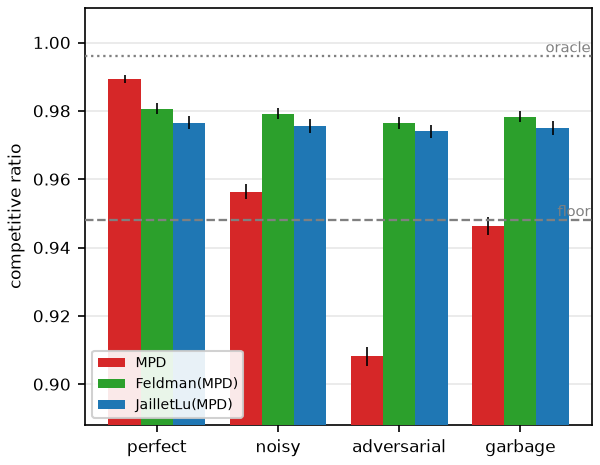
\includegraphics[width=\linewidth]{../../results/unified_benchmark_panelA.png}
\end{minipage}

\medskip
\noindent
\begin{minipage}[c]{0.62\linewidth}
\begin{tabular}{@{}lrrrr@{}}
\toprule
\emph{Panel B --- left-regular $d{=}5$} & perfect & noisy & advers. & garbage \\
\midrule
Greedy $=$ Ranking (floor) & 0.890 & --- & --- & --- \\
MinDegree (oracle) & 0.966 & --- & --- & --- \\
MPD & 0.932 & 0.906 & \textbf{0.854} & 0.888 \\
Feldman(MPD) & 0.906 & 0.902 & 0.896 & 0.900 \\
JailletLu(MPD) & 0.904 & 0.903 & 0.899 & 0.901 \\
Feldman (base) & 0.760 & --- & --- & --- \\
JailletLu (base) & 0.788 & --- & --- & --- \\
\bottomrule
\end{tabular}
\end{minipage}\hfill
\begin{minipage}[c]{0.36\linewidth}
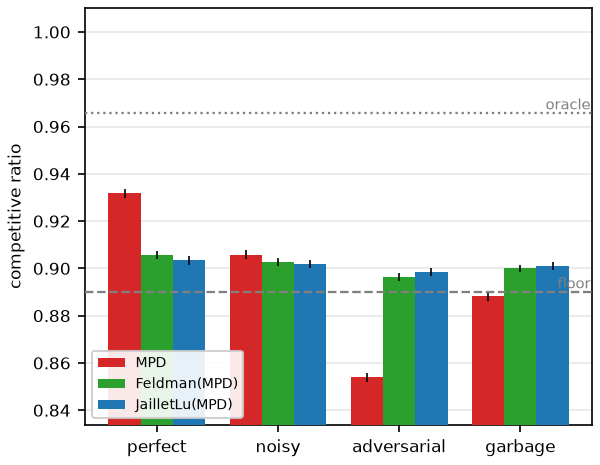
\includegraphics[width=\linewidth]{../../results/unified_benchmark_panelB.png}
\end{minipage}

\medskip
\noindent
\begin{minipage}[c]{0.62\linewidth}
\begin{tabular}{@{}lrrrr@{}}
\toprule
\emph{Panel C --- few-types $r{=}8$} & perfect & mild & bad & garbage \\
\midrule
Ranking (floor) & 0.990 & --- & --- & --- \\
MinDegree (oracle) & 0.999 & --- & --- & --- \\
FollowPrediction & 1.000 & 0.832 & 0.679 & \textbf{0.472} \\
TestAndMatch (Choo) & 1.000 & 0.984 & 0.989 & 0.990 \\
TestAndMatch (BEM) & 0.998 & 0.988 & 0.988 & 0.968 \\
Combiner \emph{(benchmark)} & 0.990 & 0.990 & 0.990 & 0.990 \\
\bottomrule
\end{tabular}
\end{minipage}\hfill
\begin{minipage}[c]{0.36\linewidth}
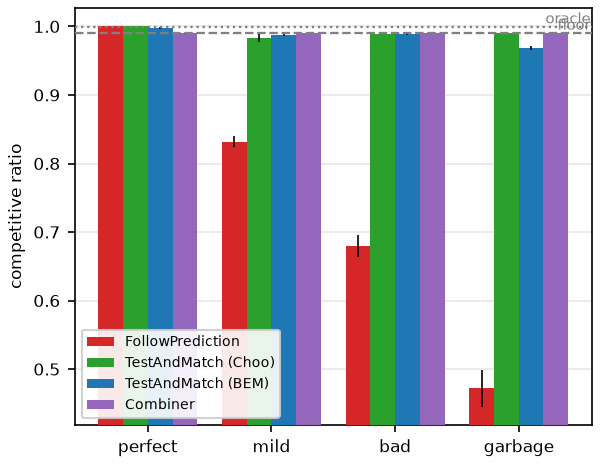
\includegraphics[width=\linewidth]{../../results/unified_benchmark_panelC.png}
\end{minipage}
\end{table}

\section{3.2 Four findings}\label{four-findings}

\revpair{\textbf{(F1) Robustness is engineered, not free: naive followers crash
below the floor.} Both unguarded prediction-followers dive under the
advice-free Ranking floor once the prediction is adversarial or garbage:
MPD falls to \(0.908 < 0.948\) (Panel A, adversarial) and
\(0.854 < 0.890\) (Panel B), and FollowPrediction collapses to
\(0.472 \ll 0.990\) (Panel C). A practitioner using either
\emph{unguarded}\revhl{revMust}{is strictly worse off than using no prediction at all.}\revhlid{revMust}{2-03}
Every \emph{robust} algorithm in the tables --- the augmentations,}{\revcard{revMust}{2-03 · P2 领域审稿人 · 必改 · 无条件断言}{%
\textbf{问题}\hspace{0.4em}strictly worse off 是无条件的，但同一张表里 MPD 在 perfect 与 noisy 两列都高于 floor。这句话能被自己的表格直接反驳。\par
\textbf{建议}\hspace{0.4em}补条件：under adversarial or garbage advice。一个从句的事。 -->}}

\revpair{\textbf{(F2) Two distinct robustness mechanisms, with different shapes.}
\emph{Structural} robustness (Feldman(MPD), JailletLu(MPD)): a
worst-case-optimal base matching carries the load and the prediction
only breaks ties, so performance is nearly \emph{flat} across quality
--- Feldman(MPD) moves only \(0.981\!\to\!0.976\) from perfect to
adversarial (Panel A). It cannot crash, but it also caps the upside (it
never reaches the \(0.996\) oracle, and sits below MPD's \(0.989\) at
perfect). \emph{Adaptive} robustness (TestAndMatch): test a sublinear
prefix, then commit --- capturing the upside when advice is good (Choo
\(1.000\) at perfect) \emph{and} holding the floor when advice is bad
(\(0.990\) at garbage). On Panel C it is the only algorithm on the upper
envelope at both ends. The two mechanisms trade consistency for
robustness in opposite ways.}{}

\revpair{\textbf{(F3) The consistency upside is small on average-case inputs; the
spread lives on the bad-advice side.} On few-types the advice-free
Ranking is already \(0.990\) and MPD-with-true-degrees is \(0.999\) ---
under \(0.01\) for \emph{any} advice to add on the good side. Every wide
gap in Panel C (\(1.000\!\to\!0.472\) for FollowPrediction; the
half-wide envelope) is a \emph{downside} gap. This is the thesis in one
panel: learning-augmented matching on typical inputs is robustness
insurance, not a performance lift --- a fact Section 7 prices: safely
capturing an upside this small would take a longer prefix than the
instance itself.}{}

\revpair{\textbf{(F4) The augmentation rescues structurally weak base
algorithms.} Feldman and Jaillet--Lu are tuned for the worst-case ratio
and are the \emph{weakest} advice-free entries on these average-case
inputs (Panel B: \(0.760\) / \(0.788\), well below Greedy's \(0.890\)).
The MPD augmentation lifts them to \(\approx 0.90\) --- the prediction
does \emph{more} for the worst-case-designed algorithms than for greedy.
\revhl{revShould}{This pairing is visible only under a}\revhlid{revShould}{2-04}}{\revcard{revShould}{2-04 · P5 审稿意见预演 · 建议 · 自我表扬}{%
\textbf{问题}\hspace{0.4em}visible only 是对自己方法论的表扬，且容易被反驳（分别做两组实验也能看到）。审稿意见里这类句子是免费靶子。\par
\textbf{建议}\hspace{0.4em}去掉 only：a pairing that a unified table makes immediate。 -->}}

\section{3.3 Takeaway}\label{takeaway}

\revpair{Read together, F1--F4 say that on average-case matching the advice-free
baseline is already near-optimal, unguarded prediction-following is
unsafe, and the value of the sophisticated algorithms is downside
protection delivered by one of two mechanisms. Sections 4--6 sharpen and
stress-test each part --- what governs the (small) loss, what the
adaptive test costs, and whether the picture survives on real graphs,
real traces, and a learned predictor --- and Section 7 proves the wall
is not an artifact but a price: a budget--stakes law that puts the
required test prefix beyond the horizon exactly where the baseline is
strong.}{}

\chapter{4. What Governs the Loss: Order-Error and ACI's
Bound}\label{what-governs-the-loss-order-error-and-acis-bound}

\revpair{MinPredictedDegree matches by ascending predicted degree, so it depends
on the predictor \(\mu\) \emph{only through the order it induces on the
resources}. Two predictors that induce the same order produce identical
matchings; a monotone rescaling of \(\mu\) changes nothing. The natural
question is therefore not ``how large is the prediction error'' but
``which \emph{order} error governs the loss,'' and how tightly. This
section answers that empirically. It also requires care: the qualitative
fact that order --- not magnitude --- matters is \emph{already theorem}
in the literature, and we are explicit about what is prior and what is
ours.}{}

\revpair{\textbf{What is already known (ACI).} Aamand, Chen \& Indyk {[}ACI22,
Appendix D{]} prove, for MinPredictedDegree on the CLV-B model, that the
matching loss relative to the true expected degrees is at most
\(n - \mathrm{LIS}(p[\mu])\), where \(p[\mu]\)\revhl{revMust}{is the true weights
ordered by}\revhlid{revMust}{3-01} \(\mu\) and \(\mathrm{LIS}\) is the longest non-decreasing
subsequence --- a pure \emph{order} quantity. In particular a monotone
(order-preserving) predictor has \(p[\mu]\) already sorted, so
\(\mathrm{LIS}=n\), \(n-\mathrm{LIS}=0\), and the loss is zero. Thus}{\revcard{revMust}{3-01 · P4 体例校对 · 必改 · 符号复用}{%
\textbf{问题}\hspace{0.4em}这里的 p 是真实权重向量，而 §2 的 p 是类型分布——两处都在讨论预测误差的语境里。核心公式因此可能被读错。\par
\textbf{建议}\hspace{0.4em}把真实权重换成 w，公式写成 n - LIS(w[mu])，并在首次出现处说明它与类型分布 p 无关。 --> *order-dependence* and *the zero-effect of a monotone bias* are ACI's results, not ours; our `systematic\_bias` error model (a monotone rescale) has Kendall-\$\textbackslash{}tau\textbackslash{}equiv 0\$ *by construction* and, consistently, leaves MPD's ratio exactly unchanged across the benchmark}}

\revpair{Our contribution is to characterize \emph{how the bound behaves} and
\emph{which order measure predicts the realized loss}. We sweep the four
structured error models across strength and record, per model and level,
three quantities on the same instances: the actual MPD matching loss,
ACI's \(n-\mathrm{LIS}\), and the normalized Kendall-\(\tau\) order
error (\textbf{Figure 1}; \(n=1000\), Zipf exponent \(1.0\), 40 trials).}{}

\revpair{\revfigure{../../results/order_vs_theory.png}{Order error, not magnitude, governs MPD's loss: (a) realized
loss sits far below the \(n-\mathrm{LIS}\) bound at every point; (b) the
four error models collapse onto the Kendall-\(\tau\) axis.}}{}

\revpair{\textbf{(i) ACI's \(n-\mathrm{LIS}\) bound is correct but very loose.}
\revhl{revShould}{The realized loss sits far}\revhlid{revShould}{3-02} below the \(n-\mathrm{LIS}\) upper bound at
every point --- by roughly \(16\times\)}{\revcard{revShould}{3-02 · P2 领域审稿人 · 建议 · 倍数口径}{%
\textbf{问题}\hspace{0.4em}没说这个倍数是怎么取的：界除以损失的均值，还是在某个误差强度上取的比。松紧程度是本节的贡献之一，审稿人需要能复核。\par
\textbf{建议}\hspace{0.4em}写明口径：ratio of the bound to the realized loss at each model's strongest corruption level。 --> (adversarial) to \$75\textbackslash{}times\$ (distribution-drift). Figure 1(a) plots loss against}}

\revpair{\textbf{(ii) \(n-\mathrm{LIS}\) saturates and cannot distinguish error
structures.} For every non-trivial error the quantity is pinned near its
maximum (\(n-\mathrm{LIS}\approx 610\)--\(673\) for \(n=1000\)), even
though the true losses differ by a factor of five across models ---
\(8.1\) (drift), \(21.6\) (random-flip), and \(41.7\) (adversarial) at
full strength. As an upper bound that is (almost) always \(\approx n\),
it carries little information about which prediction is actually more
harmful.}{}

\revpair{\textbf{(iii) Kendall-\(\tau\) is the governing order measure, and the
error models collapse onto it.} Plotting the realized loss against the
Kendall-\(\tau\) order error (Figure 1(b)), \revhl{revMust}{the four structured error
models fall on a single increasing curve}\revhlid{revMust}{3-03}: loss rises monotonically with
Kendall-\(\tau\) (\(0.29\to0.50\to1.0\) for drift, random-flip,
adversarial, tracking \(8.1\to21.6\to41.7\) in loss), with
\texttt{systematic\_bias} pinned at \(\tau=0\) and zero loss. The
quantity that \emph{predicts} the loss --- and unifies the error models
--- is the Kendall-\(\tau\)}{\revcard{revMust}{3-03 · P2 领域审稿人 · 必改 · 视觉断言缺量化}{%
\textbf{问题}\hspace{0.4em}这是本节的正面结论，支撑它的只有一句对图的目视描述。审稿人一定会要一个数。\par
\textbf{建议}\hspace{0.4em}给统计量。四个模型全部误差水平合并（44 个点）的实测值是 Spearman rho = 0.979、Pearson r = 0.992，各非退化模型内部均不低于 0.97——直接写进正文即可。}
\revcard{revShould}{3-04 · P1 领域外审稿人 · 建议 · 度量未定义}{%
\textbf{原文}\hspace{0.4em}\textquotedblleft the normalized Kendall-tau order error\textquotedblright\par
\textbf{问题}\hspace{0.4em}normalized 的归一化方式没说：0 表示完全一致、1 表示完全反序吗。第 6 节还要拿它跨数据集比较。\par
\textbf{建议}\hspace{0.4em}给一句：reported on [0,1], where 0 means the predicted order is exactly right and 1 that it is exactly reversed。 -->}}

\revpair{\textbf{Takeaway (and scope).} We do not claim that order, rather than
magnitude, governs MPD --- ACI's Appendix D establishes that, and the
zero-effect of a monotone bias with it. What we add is a precise
empirical characterization: ACI's \(n-\mathrm{LIS}\) bound is loose by
one to nearly two orders of magnitude and saturates, whereas
Kendall-\(\tau\) predicts the realized loss and unifies the four error
structures onto one curve. This both sharpens the theory's practical
content and justifies the single order-error axis we use when we
stress-test the predictor on real data (Section 6).}{}

\chapter{5. Test-and-Fallback in
Depth}\label{test-and-fallback-in-depth}

\revpair{The test-and-fallback algorithms are the paper's adaptive robustness
mechanism, and the object of the theory in Section 7. This section gives
their first empirical study: the robustness envelope they achieve
(§5.1), a counter-intuitive failure of the acceptance threshold (§5.2),
its recalibration and the resolution limit that recalibration exposes
(§5.3) --- the empirical face of the budget--stakes law we prove in
Section 7 --- a \textbf{constant-free payoff-testing rule} that the law
suggests and that avoids both threshold pathologies (§5.4), and the
dynamic combiner benchmark that explains \emph{commit-once} (§5.5).
Throughout, the \(\ell_1\) test is the empirical-\(\ell_1\)
proof-of-concept the original authors also fall back to (Section 2.2).}{}

\section{5.1 The robustness envelope}\label{the-robustness-envelope}

\revpair{We sweep advice error \(\ell_1(p,q)\) on few-types instances
(\(n=2000\), \(r=8\), prefix \(k=200\), 40 trials) and compare blind
FollowPrediction, TestAndMatch (Choo and BEM variants), and the Ranking
floor (\textbf{Figure 2}). The picture is textbook. FollowPrediction
degrades \emph{linearly}, from \(1.000\) at perfect advice to \(0.453\)
at \(\ell_1\!\approx\!1.1\) --- well \emph{below} the advice-free floor
(\(\approx 0.99\)). TestAndMatch instead stays on the \textbf{upper
envelope}: it captures the benefit when advice is good and, when advice
is bad, \revhl{revMust}{its prefix test rejects it and it falls back to Ranking, never
crashing}\revhlid{revMust}{4-01} (BEM \(0.998\to0.969\); Choo \(1.000\to0.991\) across the same
sweep). This is the adaptive counterpart of the structural robustness of
Section 3: the engineered mechanism}{\revcard{revMust}{4-01 · P2 领域审稿人 · 必改 · 全称断言}{%
\textbf{问题}\hspace{0.4em}never 是全称量词，证据是一条误差 sweep、一个图族、40 次重复。\par
\textbf{建议}\hspace{0.4em}限定到证据范围：it does not fall below the advice-free floor at any point of this sweep。真正的全称结论交给 §7 的定理承担。 -->}}

\revpair{\revfigure{../../results/choo_bem_envelope.png}{The robustness envelope: blind FollowPrediction crashes below
the advice-free floor as advice error grows; TestAndMatch stays on the
upper envelope.}}{}

\section{5.2 A threshold that is too lenient on average-case
inputs}\label{a-threshold-that-is-too-lenient-on-average-case-inputs}

\revpair{What does the ``test then maybe fall back'' machinery cost, and does a
better test make a better decision? We sweep the prefix (testing) size
\(k\) at \emph{borderline} advice (\(\eta=0.15\), true
\(\ell_1\!\approx\!0.16\)) --- the regime where the test must work
hardest (\textbf{Figure 3}). Counter-intuitively, \textbf{a larger, more
accurate test makes the \emph{worse} decision}: as \(k\) grows
\(25\to100\to200\to800\), the ratio \emph{falls} \(0.992\to0.981\to
0.969\to0.956\) and the misjudgement rate (against an empirical oracle:
should we have followed, given that following actually underperformed
the baseline here?) \emph{rises} \(0.00\to0.13\to0.33\to0.60\).}{}

\revpair{\revfigure{../../results/choo_bem_prefix.png}{Testing cost at borderline advice: under the
worst-case-calibrated threshold, a larger and more accurate prefix test
makes the \emph{worse} decision.}}{}

\revpair{The mechanism is a real and reportable finding. The Choo/BEM acceptance
threshold \(\tau\) \revhl{revMust}{is calibrated to the}\revhlid{revMust}{4-02} \emph{worst-case} baseline
\(\beta\approx0.696\). But on these average-case instances the baseline
is \(\approx0.99\) (Section 3, F3), so the \emph{empirical} break-even
--- the advice error at which following stops beating the baseline ---
sits at \(\ell_1\approx0\), far below \(\tau\). A small, noisy prefix
over-estimates \(\ell_1\) and \emph{accidentally rejects} the borderline
advice, landing on the strong Ranking floor; a large, accurate prefix
correctly measures \(\ell_1\approx0.16<\tau\) and so \textbf{accepts}
the mildly-bad advice the worst-case threshold deems acceptable --- and
underperforms the baseline. On strong-baseline inputs the
worst-case-calibrated threshold is too \emph{lenient}, and improving the
test's}{\revcard{revMust}{4-02 · P1 领域外审稿人 · 必改 · 常数无出处}{%
\textbf{问题}\hspace{0.4em}0.696 凭空出现。领域外审稿人会问它是哪来的、为什么不是 1-1/e。它是本节机制解释的支点。\par
\textbf{建议}\hspace{0.4em}补半句出处：随机到达序下 Ranking 的最坏情况比值，也是 Choo 等人给阈值取的值，并引 [Choo24]。 -->}}

\section{5.3 Recalibration, and the resolution limit it
exposes}\label{recalibration-and-the-resolution-limit-it-exposes}

\revpair{The natural fix is to recalibrate \(\tau\) to the \emph{measured}
baseline \(\hat\beta\) (the mean empirical Ranking ratio on a small
calibration sample) rather than the worst-case \(\beta\). On the same
instances this eliminates the pathology: at borderline advice the
worst-case threshold's misjudgement climbs \(0.03\to1.00\) as the prefix
grows and its ratio drops to \(0.920\), whereas the recalibrated
threshold holds misjudgement \(=0.00\) at every prefix size and ratio
\(\approx0.986\) --- a larger prefix no longer hurts.}{}

\revpair{But recalibration exposes a deeper, honest limit. At \emph{perfect}
advice (\(\ell_1=0\)) the worst-case threshold scores \(1.000\) (it
accepts and follows), while the recalibrated one scores only \(0.987\):
the recalibrated threshold \(\tau\approx 2(1-\hat\beta)\approx 0.028\)
is \emph{smaller than the empirical-\(\ell_1\) estimator's own noise
floor} (\(\approx 0.05\)--\(0.13\) \revhl{revShould}{at this prefix and support)}\revhlid{revShould}{4-03}, so the
test can never confidently \emph{accept} --- it rejects everything,
including perfect advice, and effectively always plays the baseline. In
other}{\revcard{revShould}{4-03 · P2 领域审稿人 · 建议 · 估计量缺说明}{%
\textbf{问题}\hspace{0.4em}噪声底给了区间但没说怎么估的、随什么变化。它是 §5.3 到 §7 的桥。\par
\textbf{建议}\hspace{0.4em}补一句定义：完美建议下长度 k 前缀的类型频率与真实直方图的 l1 距离，即纯采样噪声，随 k 增大而下降。 -->}}

\revpair{\begin{quote}
On strong-baseline instances, no practical empirical-\(\ell_1\)
threshold can both capture the consistency upside and stay safe: the
upside is tiny (the baseline is already \(\approx\mathrm{OPT}\)) and
sits \emph{below the estimator's resolution}. The worst-case threshold
over-accepts (§5.2); the recalibrated threshold over-rejects; and a
better tester only follows whichever threshold more faithfully.
\end{quote}}{}

\revpair{Section 7 turns this phenomenon into a two-sided law. The resolution
limit above is specific to the empirical-\(\ell_1\) statistic --- §7.7
shows that class is blind for a structural reason (the plug-in distance
saturates at \(k \ll r\) regardless of advice quality) --- but the
deeper point holds for \emph{any} test on a sublinear prefix: the
follow/fallback decision costs a prefix of
\(\tilde\Theta(\sigma^2/g^2)\) --- baseline slack over squared stakes
--- and on strong-baseline instances like these the stakes are so small
that the price exceeds the horizon. Section 5 is the empirical shadow;
Section 7 is the law. But the resolution limit is a property of the
\emph{statistic}, not of testing itself --- the next subsection builds
the rule the law suggests, and it behaves differently.}{}

\section{5.4 Testing the payoff instead: a decision rule with no
constants}\label{testing-the-payoff-instead-a-decision-rule-with-no-constants}

\revpair{The budget--stakes law identifies the decision-relevant statistic: not
the advice's distance to the truth, but the \emph{payoff} of following
it. We implement this as \textbf{DirectionalTest-and-Match}: the same
commit-once protocol (Mimic the prefix, decide once), with the
\(\ell_1\) threshold replaced by a plug-in payoff comparison. From the
prefix's empirical type distribution \(\hat p\), the value of continuing
to Mimic has an exact closed form,
\(V_{\mathrm{mimic}}(\hat p)=\sum_l \min(n\hat p_l, s_l)\), where
\(s_l\) is the number of offline slots the advice matching allocates to
type \(l\); the value of the Ranking baseline,
\(V_{\mathrm{rank}}(\hat p)\), is estimated by simulating Ranking on the
\emph{public} type graph under the same distribution. The rule follows
iff the corrected difference is nonnegative. Two implementation findings
are part of the paper's message. First, the naive plug-in is
\emph{biased}: \(V_{\mathrm{mimic}}\) is concave, so honest sampling
noise in \(\hat p\) drags the estimate down at the capacity kinks
(Jensen), and an uncorrected rule rejects even perfect advice; a
parametric bootstrap anchored at \(\hat p\) removes the bias (anchoring
at the advice instead over-corrects exactly for mildly bad advice, whose
true distribution sits in the locally linear region). Second, the rule
uses \textbf{no problem constants}: no worst-case \(\beta\), no
threshold \(\tau\) --- every quantity is computed from the prefix and
public information. A public-information early exit (fall back without
spending the prefix when even a \emph{correct} advice would not beat the
baseline) restores parity with Choo et al.'s \(\hat n/n\le\beta\) exit.}{}

\revpair{\textbf{Figure 4} repeats the envelope sweep with the payoff rule added,
against both the worst-case and the recalibrated thresholds. The three
rules now separate cleanly. At mildly bad advice --- where the
worst-case threshold follows the crash (\(0.948\) and \(0.937\) at
\(\ell_1\approx0.10\) and \(0.21\), misjudging \(100\%\) and \(63\%\) of
instances) --- the payoff rule stays at the floor (\(0.989/0.990\),
misjudgement \(3\%/0\%\)). At perfect advice --- where the recalibrated
threshold \emph{never} follows (misjudgement \(100\%\), §5.3) --- the
payoff rule captures the upside in \({\sim}40\%\) of instances and lands
safely on the floor otherwise. That partial capture is the honest
ceiling, not a defect: the family's upside (\(\approx0.02\)) lies below
the resolution \emph{any} rule can achieve at \(k=200\) --- by the
budget--stakes scaling of Section 7, \revhl{revMust}{with this family's payoff estimator
carrying per-sample variance of order one, resolving stakes of}\revhlid{revMust}{4-04} \(0.02\)
takes \(k \approx 1/0.02^2 = 2500 > n\) --- the law binds our rule too,
and the right behavior at}{\revcard{revMust}{4-04 · P2 领域审稿人 · 必改 · 把 sigma\textasciicircum{}2 悄悄设成 1}{%
\textbf{问题}\hspace{0.4em}§7 的预算是 sigma\textasciicircum{}2/g\textasciicircum{}2，这里直接写成 1/g\textasciicircum{}2，等于把 sigma\textasciicircum{}2 取成 1 而只用一个从句带过。审稿人会问：benchmark 家族的 sigma\textasciicircum{}2 到底是多少？这是把定理用到自己算法上的唯一一处，不能含糊。\par
\textbf{建议}\hspace{0.4em}把 sigma\textasciicircum{}2 的取值（或它在该家族上的量级估计）写出来，公式写成 k approx sigma\textasciicircum{}2/g\textasciicircum{}2 并代入具体数字。 -->}}

\revpair{\revfigure{../../results/directional_envelope.png}{The envelope sweep with the payoff rule added: the worst-case
threshold follows the crash at mildly bad advice, the recalibrated
threshold never captures at perfect advice, and the constant-free payoff
rule tracks the upper envelope within the resolution the budget--stakes
law allows.}}{}

\revpair{\textbf{Figure 5} is the head-to-head that summarizes the section. At
borderline advice (\(\eta=0.15\)), growing the prefix from \(k=25\) to
\(800\) drives the worst-case threshold's misjudgement \emph{up} from
\(0.07\) to \(1.00\) (ratio \(0.987\to0.922\)) --- §5.2's pathology in
full --- while the payoff rule's misjudgement falls monotonically from
\(0.53\) to \(0.00\) (ratio \(0.954\to0.991\)). More data helps if and
only if the statistic being sharpened is the decision-relevant one; the
recalibrated threshold is flat-safe here only because it always rejects.
In one sentence: \textbf{test the payoff, not the prediction.}}{}

\revpair{\revfigure{../../results/directional_prefix.png}{Borderline advice (\(\eta=0.15\)): as the prefix grows, the
worst-case threshold's misjudgement rises to \(1.0\) while the payoff
rule's falls to \(0.0\) --- more data helps exactly when the statistic
is the decision-relevant one.}}{}

\revpair{The honest costs: when advice is bad but not worthless-if-true, the
payoff rule pays the same prefix cost as its competitors (\(\approx1\)
point at \(k/n=0.1\); the early exit rarely fires on spiky advice), and
its simulation budget --- a handful of Ranking runs on the type graph
--- is computation, not samples. All numbers: 30 paired trials per
point, seed-fixed (\texttt{scripts/run\_directional\_test.py},
\texttt{results/directional\_test.json}).}{}

\section{5.5 The dynamic combiner is dominated, and shows why matching
needs
test-then-commit}\label{the-dynamic-combiner-is-dominated-and-shows-why-matching-needs-test-then-commit}

\revpair{Finally we benchmark the Chłędowski-style dynamic combiner (Section 2.2)
to contextualize the \emph{commit-once} structure of test-and-fallback.
In its intended robust tuning the combiner sits exactly on the floor
(\(0.990\) across all advice quality on few-types): it never crashes,
but captures \emph{none} of the consistency upside --- strictly
dominated by TestAndMatch on the good-advice side and equal to it on the
bad side.}{}

\revpair{More instructively, an \emph{eager} combiner that switches experts
mid-stream reveals a penalty specific to irrevocable problems. With
perfect advice, \revhl{revMust}{eager switching scores}\revhlid{revMust}{4-05} \(0.927\) --- \emph{below both}
the pure follower (\(1.000\)) and the pure baseline (\(0.958\); verified
in \texttt{tests/test\_combiner\_small.py}) --- because switching from
Ranking to Mimic mid-run lands the}{\revcard{revMust}{4-05 · P7 复现审稿人 · 必改 · 用单元测试当证据}{%
\textbf{问题}\hspace{0.4em}论文正文的数字引用了一个单元测试文件。实际规模是 n=600、r=6、单个种子、不做平均——全节其他数字都有实验设置，只有这一处没有，且它支撑的是」为何必须 test-then-commit」这一结论。\par
\textbf{建议}\hspace{0.4em}写明它的地位与规模：a single-instance mechanism check (n=600, r=6, one seed, no averaging)，或升级为一次带置信区间的正式实验。脚本路径移到复现附录。 --> committed matching in an *incompatible hybrid*: the Mimic plan's slots are already half-consumed by the Ranking phase, and the Ranking progress is abandoned. In an irrevocable problem the follow/fallback decision must be made *before* the bulk of the commitments, not adapted across them — which is precisely why Choo/BEM test on a prefix and then *commit*, rather than switching dynamically as the caching-style combiner does. The dynamic combiner that is cheap worst-case insurance for caching does not port cleanly to}}

\chapter{6. External Validity}\label{external-validity}

\revpair{Sections 3--5 are on synthetic graphs with a synthetic error knob. Is
the picture real? We stress it three ways: a genuine, cheap predictor on
a real request trace (§6.1); the six real-world graphs (§6.2); and
whether \emph{learning} the predictor changes anything (§6.3).}{}

\section{6.1 A real, cheap predictor}\label{a-real-cheap-predictor}

\revpair{We replace the synthetic error knob with the cheapest realistic
predictor: last-window historical statistics. Real Wikipedia daily
pageviews give a live day (the truth) and earlier days (a 1-, 7-, or
30-day-stale forecast), so the prediction error is genuine temporal
drift; we map the trace onto a fixed serving topology and \revhl{revMust}{consume the
forecast}\revhlid{revMust}{5-01} through the degree route (MPD) (\textbf{Figure 6};
\texttt{docs/REAL\_PREDICTOR.md}).}{\revcard{revMust}{5-01 · P7 复现审稿人 · 必改 · 指向仓库内部文档}{%
\textbf{问题}\hspace{0.4em}第 6 节正文三次把读者指向仓库里的 markdown 笔记。审稿人只有 PDF，这些指向对他们等于不存在；而它们支撑的是本节的主要数字。\par
\textbf{建议}\hspace{0.4em}凡支撑正文数字的，摘进复现附录；其余删掉。脚本路径可以保留（artifact 里有），docs/*.md 不行。}}

\revpair{\revfigure{../../results/real_predictor.png}{A cheap historical-count predictor on the Wikipedia trace:
near-oracle ratio at every staleness level, never below the advice-free
floor.}}{}

\revpair{Three facts emerge, all favorable and all honest. First, \textbf{the
cost premise does not bite}: the predictor is a linear-time count
(\(\mu = A\,p\) over historical frequencies), \(0.108\) ms per instance
--- about \(2\%\) of the cost of computing \(\mathrm{OPT}\) once --- not
an ML inference. Second, \textbf{the benefit is real, partial, and never
harmful}: a stale forecast captures \(27\%\)--\(68\%\) of the achievable
oracle gap (falling with staleness) and \emph{always} stays above the
forecast-free baseline (\(0.938\)--\(0.957\) vs \(0.923\)--\(0.925\),
even at 30 days). Third, and explaining why, \textbf{topology
aggregation makes the cheap predictor order-faithful}: the induced
degree predictor's order error is only Kendall-\(\tau\approx
0.19\)--\(0.32\), roughly \emph{half} the raw type-histogram's
(\(0.38\)--\(0.49\)) --- and since MPD depends only on order (Section
4), the aggregated degree route survives real drift. Consuming the
\emph{same} stale forecast through the raw histogram instead is
catastrophic: blind FollowPrediction collapses to \(0.68\to0.36\), far
below the \(\approx0.92\) baseline --- exactly what the robust
algorithms of Sections 3 and 5 are for.}{}

\section{6.2 Six real-world graphs}\label{six-real-world-graphs}

\revpair{We re-run the degree-prediction roster of Section 3 on the six
Network-Repository graphs (two Facebook social, two C. elegans
biological, two economic input-output), across the same quality columns,
with 95\% CIs (\textbf{Figure 7};
\texttt{docs/REALWORLD\_ROBUSTNESS.md}).}{}

\revpair{\revfigure{../../results/realworld_robustness.png}{The six real-world graphs: unguarded following falls below the
advice-free floor on every graph, and the augmentation restores safety
--- the benchmark's findings are universal, not generator artifacts.}}{}

\revpair{The two load-bearing findings are universal. \textbf{F1 holds on all six
graphs}: naive MPD \revhl{revMust}{fed an adversarial predictor falls}\revhlid{revMust}{5-02} \emph{below} the
Ranking floor everywhere --- by \(0.07\) (Caltech36: \(0.843<0.913\)) to
\(0.11\) (CE-PG: \(0.782<0.883\)). **\revhl{revMust}{F3 is universal and}\revhlid{revMust}{5-03}}{\revcard{revMust}{5-02 · P2 领域审稿人 · 必改 · 算术与断言}{%
\textbf{问题}\hspace{0.4em}两处问题。其一，0.883-0.782 = 0.101，四舍五入是 0.10 不是 0.11，而括号里的两个数就在同一句里，审稿人一眼能验算。其二，最小跌幅其实是 Reed98 的 0.063，不是 Caltech36 的 0.070。\par
\textbf{建议}\hspace{0.4em}改成 by 0.06 (Reed98) to 0.10 (CE-PG)，或保留 Caltech36 作为例子但把区间端点写对。}
\revcard{revMust}{5-03 · P2 领域审稿人 · 必改 · universal}{%
\textbf{问题}\hspace{0.4em}universal 用在六个图的样本上过强，而紧接着就要说 F2 在其中两个图上只是部分成立。\par
\textbf{建议}\hspace{0.4em}改成 holds on all six graphs we tested；机制解释（上升空间在基线最强处最小）才是这一节的价值。 --> confirms its own logic**: the consistency upside (best prediction algorithm at perfect advice, over the floor) is small everywhere (mean \$+0.049\$; range \$+0.022\$–\$+0.077\$), and it is *smallest exactly where the baseline is strongest* — the two dense economic graphs,}}

\revpair{The structural-robustness finding \textbf{F2 holds qualitatively on all
six} (the augmentations are always less sensitive to prediction quality
than naive MPD) and \emph{strictly} on the four social/bio graphs
(augmentation spread \(0.22\)--\(0.29\times\) MPD's); on the two dense
economic graphs the protection is only \emph{partial} --- the
augmentation cushions the adversarial drop (beause: \(0.939\) vs naive
MPD's \(0.893\)) but cannot fully clear the unusually high \(0.965\)
floor, dipping \(\approx0.03\) below it (spread ratio
\(0.53\)--\(0.55\)). \revhl{revShould}{This econ boundary is instructive rather than a
failure}\revhlid{revShould}{5-04}: those graphs are so dense that matching is nearly trivial
(Ranking \(\approx0.97\), MinDegree \(=1.00\)), so there is neither
upside to capture (F3) nor much downside to protect --- the mechanisms
compress together}{\revcard{revShould}{5-04 · P5 审稿意见预演 · 建议 · 自我辩护}{%
\textbf{问题}\hspace{0.4em}遇到不利结果先给自己定性，是审稿人最敏感的写法之一，反而会让人多看两眼这个边界。后面的解释本身已经充分。\par
\textbf{建议}\hspace{0.4em}删掉这句评价，直接给解释：那两个图太稠密，匹配近乎平凡，既无上升空间可抓也无多少下行需保护——这是 F3 的机制在起作用，不是它的例外。 --> where robustness does not matter. Finally, F4 is *dramatic* here: the worst-case-designed Feldman/Jaillet–Lu are the weakest advice-free entries on the econ graphs (\$0.73\$–\$0.77\$),}}

\section{\texorpdfstring{6.3 Does \emph{learning} the predictor help? A
negative
result}{6.3 Does learning the predictor help? A negative result}}\label{does-learning-the-predictor-help-a-negative-result}

\revpair{Because MPD consumes the predictor only through its order (Section 4),
one might train the predictor with an order-aware (rank) loss rather
than regression. We test this and report an honest negative
(\texttt{docs/RANK\_LEARNING\_M0\_M3.md}). With \emph{deliberately
divergent} synthetic features --- one carrying magnitude, one carrying
order --- rank-training does beat regression sharply (matching ratio
\(0.989\approx\) oracle vs \(0.974\), with rank-training having
\emph{worse} regression error but better order). But the advantage is
gated by two things that both vanish in practice: it is zero when
features do not induce an order/magnitude divergence and zero on easy
instances (F3 again), peaking at only \(+1.3\%\) on synthetic graphs;
and, decisively, \textbf{on real temporal features it disappears} ---
trained on lagged counts from real serving traces, the rank- and
regression-trained predictors produce \emph{identical} order
(Kendall-\(\tau\) \(0.126\) vs \(0.126\)) and identical matching ratio,
\revhl{revShould}{across every topology and}\revhlid{revShould}{5-05}}{\revcard{revShould}{5-05 · P2 领域审稿人 · 建议 · 负结果的覆盖面}{%
\textbf{问题}\hspace{0.4em}这是本节最有分量的负结果，支撑它的是一句 every ... we tried，但配置清单没给。负结果的说服力全在覆盖面。\par
\textbf{建议}\hspace{0.4em}把实际配置写进正文一句：150 个上下文长度类型、500 个度数为 8 的副本、40 个窗口、三个滞后特征、60/40 划分；若确实扫过多组拓扑与滞后，把清单也列出来。 --> lag we tried. The dissociation that powers order-aware training is a property of engineered features, not of realistic ones. The lesson reinforces the thesis: once a predictor is order-faithful — which a cheap historical count already is (§6.1) — neither a better}}

\section{Summary}\label{summary}

\revpair{On real predictors, real graphs, and a learned predictor, the same wall
stands: the advice-free baseline is near-optimal, unguarded following is
unsafe, and predictions buy downside protection rather than performance.
Having established the wall empirically across every setting we could
reach, we now prove it is necessary.}{}

\revpair{{[}PROOF STATUS --- for the authors, delete before submission{]} The
earlier draft stated a sublinear-test impossibility for ANY rule at k =
o(n/log n) via a reduction to tolerant identity testing. That theorem is
FALSE --- attempting the witness step refuted it (see
docs/T1\_WITNESS\_GAP.md): on the cell family the follow-payoff equals
half the mean of a per-sample observable, so a directional rule succeeds
at k = O(log n). This section now states what is true instead: a sharp
budget--stakes law (Theorem 1, both halves elementary ---
Bernstein/Hoeffding upper, Hellinger + Lemma 1 lower). Lemma 1 and the
affine law carry over unchanged. GENERALIZED 2026-07-28: heterogeneous
profiles (theta\_i, eps\_i) + magnitude-free achievability, organized
around the specialist mass sigma\^{}2 = sum theta\_i/N with the exact
identity 1-rho\_base = sigma\^{}2/2; verified by
scripts/verify\_budget\_stakes\_hetero.py (see
docs/T1\_HETERO\_GENERAL.md). Remaining before submission (single-author
as of 2026-07-28): the author's own line-by-line verification of this
section; typeset the two short proofs in the appendix. Novelty pass DONE
2026-07-29 (docs/NOVELTY\_PAYOFF\_TEST.md) --- no payoff-testing
acceptance rule found in the adjacent lines; positioning debts
(test-before-trust, data-driven selection, Wald) paid in the intro
paragraph and §9.}{}

\revpair{Differentiation to defend (put up front): Choo's threshold τ=2(n̂/n−β)−ε
couples to the baseline β CONSTRUCTIVELY; our lower bound is
information-theoretic (any prefix rule). And our positive result says
the field's ℓ₁-testing lens is the wrong statistic on average-case
inputs --- the decision-relevant functional (the payoff) is
exponentially cheaper to test than the distribution distance.
--\textgreater{}}{}

\chapter{7. A Budget--Stakes Law: What a Sublinear Test Can and Cannot
Buy}\label{a-budgetstakes-law-what-a-sublinear-test-can-and-cannot-buy}

\revpair{Every experiment above met the same wall: on average-case matching the
advice-free baseline is near-optimal, so predictions buy robustness
insurance rather than performance, and --- for the test-and-fallback
algorithms --- no acceptance threshold both captures the (tiny) upside
and stays safe (§5.3). This section quantifies the wall. The result is a
two-sided \textbf{budget--stakes law}: on a natural instance family,
deciding whether to follow the advice requires a prefix of length
\(k^* = \tilde\Theta(\sigma^2/g^2)\) --- the instance's specialist mass
(exactly twice its baseline slack) divided by the squared stakes \(g\)
--- and this is \emph{sharp}: below \(k^*\) \textbf{no}\revhl{revMust}{decision rule
whatsoever can be simultaneously consistent and robust (Theorem}\revhlid{revMust}{6-01} 1(i)),
while at \(k^*\) an explicit, embarrassingly simple rule succeeds
(Theorem 1(ii)). The corollary is the wall: stakes are capped by the
baseline slack, so on strong-baseline instances the required prefix
exceeds the entire horizon --- any upside smaller than
\(\approx 2\sqrt{(1-\rho_{\mathrm{base}})/n}\) is uncapturable at
\emph{every} \(k\le n\), and the upsides we measured in §3--§5 sit in
exactly that range.}{\revcard{revMust}{6-01 · P2 领域审稿人 · 必改 · sharp 的条件被省略}{%
\textbf{问题}\hspace{0.4em}Theorem 1(i) 给的不可能性门槛是 k = o(1/(eps\_W * g))，不是 o(sigma\textasciicircum{}2/g\textasciicircum{}2)；两者只在 Cauchy-Schwarz 那一步的条件下相接，而 §7.8 承认在低信号 sliver 上可差 sigma\textasciicircum{}2*eps\_W/g 倍。本节开头把 sharp 说成无条件的，审稿人读到 §7.8 会认为前面在过度宣称。\par
\textbf{建议}\hspace{0.4em}本节开头就把条件写出来：sharp up to logarithms whenever the stakes are carried, at comparable signal levels, by a constant fraction of the specialist mass；并直接指向 §7.8 的开放情形。}}

\revpair{En route we record an honest negative of independent interest (§7.7):
the natural conjecture --- that the \(\tilde\Theta(r/\log r)\) hardness
of \emph{tolerant distribution testing} {[}CJKL22, VV11, JHW18{]} makes
the follow/fallback decision itself hard for any rule at sublinear \(k\)
--- is \textbf{false}. The advice's \emph{distance} \(\ell_1(p,q)\) is
indeed hard to test, and the empirical-\(\ell_1\) rules the field
actually uses {[}Choo24, BEM26{]} are provably blind at \(k \ll r\); but
the decision-relevant functional is the \emph{payoff} of following,
which on decomposable instances collapses to a per-sample observable.
Testing the payoff is exponentially cheaper than testing the prediction.}{}

\revpair{\textbf{Relation to prior work.} Choo et al.~{[}Choo24{]} and
Burathep--Erlebach--Moses {[}BEM26{]} give \emph{upper} bounds
(algorithms) in this model and no statistical lower bound; Choo et al.'s
Thm 3.1 is the generic adversarial trade-off (no algorithm is
\(1\)-consistent and \(>\tfrac12\)-robust), driven by adversarial
instances, not by the resolution of a sublinear test. Their acceptance
threshold \(\tau = 2(\hat n/n-\beta)-\varepsilon\) couples to the
baseline \(\beta\) \emph{constructively}; Theorem 1(i) is the
information-theoretic counterpart --- it binds \emph{every} measurable
rule on the prefix. The consistency/robustness lower bounds elsewhere in
the with-predictions literature {[}WZ20{]} are problem-intrinsic Pareto
frontiers, not gated by a test. Tolerant-testing sample complexity
{[}CJKL22{]} enters our story twice, both times off the critical path:
it explains \emph{why} the field's \(\ell_1\)-threshold rules are blind
(§7.7), and its hard instances are exactly what our payoff identity
(Lemma 2) sidesteps. To our knowledge, both the budget--stakes law and
the observation that payoff-testing strictly separates from
distance-testing in an online algorithm are new. A dedicated pass over
the adjacent lines (§9) found none testing the payoff: the
\emph{test-before-trust} program of Choo, Gouleakis and coauthors
{[}Choo24, BCJG25{]} validates advice by distributional distance
throughout --- exactly the statistic §7.7 shows is the wrong one on
average-case inputs; switching frameworks {[}Chl21, ASSS25{]} switch
dynamically on prediction quality or regret rather than committing on a
payoff test, and matching's irrevocability breaks them (§5.5);
data-driven algorithm selection {[}GR17, Bal20{]} chooses among
algorithms from samples of \emph{whole instances} with observable
per-instance performance, whereas here a single instance's prefix must
reveal a policy's full-horizon value --- which is what the payoff
identity provides; and the \(1/g^2\) budget echoes classical sequential
analysis {[}Wald47{]}, whose engine --- not its novelty --- Lemma 2
imports into matching.}{}

\section{7.1 The test-and-fallback
class}\label{the-test-and-fallback-class}

\revpair{Fix an instance family and a budget \(k=o(n)\). A
\textbf{test-and-fallback} algorithm \(A_k\) observes the first \(k\)
arrivals \(X_{1:k}\) and the advice \(\sigma\), outputs a (possibly
randomized) decision \(D\in\{\mathsf{Follow},\mathsf{Fallback}\}\) as a
function of \((X_{1:k},\sigma)\), and thereafter Mimics \(\sigma\) if
\(D=\mathsf{Follow}\) and runs the advice-free baseline \(B\) (Ranking)
otherwise. Because \(k=o(n)\), the prefix's own contribution to the
ratio is \(O(k/n)=o(1)\), absorbed below. Write \(\rho_{\mathrm{base}} =
\mathbb E[B]/\mathrm{OPT}\) for the baseline strength,
\textbf{consistency} for the ratio under good advice, and
\textbf{robustness} for the ratio under adversarial advice.}{}

\section{7.2 The master trade-off
(rigorous)}\label{the-master-trade-off-rigorous}

\revpair{\begin{quote}
\textbf{Lemma 1.} Let \(G,\mathrm{Bd}\) be two instance distributions
sharing the \emph{same} advice \(\sigma\), with prefix laws
\(\mathcal L_G,\mathcal L_{\mathrm{Bd}}\) and
\(\gamma_k:=\mathrm{TV}(\mathcal L_G,\mathcal L_{\mathrm{Bd}})\).
Suppose following \(\sigma\) gains \(\delta\) under \(G\) and loses
\(\Delta\) under \(\mathrm{Bd}\) relative to \(B\). Parameterize \(A_k\)
by the fraction \(\eta_c\) of the upside it forgoes under \(G\) and its
robustness loss \(\eta_r\Delta\) under \(\mathrm{Bd}\). Then
\[(1-\eta_c)\;\le\;\eta_r+\gamma_k+o(1).\]
\end{quote}}{}

\revpair{\emph{Proof.} Conditioning on \(D\) under \(G\),
\(\mathbb E_G[A_k]/\mathrm{OPT} = P_G(\mathsf F)\,
\mathbb E_G[\mathrm{Mimic}]/\mathrm{OPT} + P_G(\mathsf R)\rho_{\mathrm{base}} \pm o(1) \ge
\rho_{\mathrm{base}} + \delta\,P_G(\mathsf F)-o(1)\), so the captured
upside \((1-\eta_c)\delta\) forces \(P_G(\mathsf F)\ge 1-\eta_c-o(1)\).
Symmetrically \(P_{\mathrm{Bd}}(\mathsf F)=\eta_r
+o(1)\). Since \(D\) is a function of \((X_{1:k},\sigma)\) and
\(\sigma\) is identical,
\(|P_G(\mathsf F)-P_{\mathrm{Bd}}(\mathsf F)|\le\gamma_k\); chaining
gives the claim. \(\qed\)}{}

\revpair{With an \emph{uninformative} prefix (\(\gamma_k=o(1)\)) one cannot be
both near-fully-consistent (\(\eta_c\to0\)) and robust (\(\eta_r\to0\)).
Everything below is a computation of how large \(k\) must be before the
prefix becomes informative --- and (the half the earlier draft missed)
of how \emph{small} a \(k\) already suffices.}{}

\section{7.3 The construction and the affine
law}\label{the-construction-and-the-affine-law}

\revpair{The family is a disjoint union of \(m\) independent
\textbf{rare-resource cells}, each over a distinct type-pair, so the
support is \(r=\Theta(m)\) and (at \(m = \Theta(n)\)) each type is seen
\(O(1)\) times. Cell \(i\) has resources \(\{a_i,b_i\}\), a flexible
request (neighborhood \(\{a_i,b_i\}\)) that must be routed before a
specialist (\(\{a_i\}\) or \(\{b_i\}\), present with probability
\(\theta_i\)) is seen; the right route depends on the future specialist.
The profile \(\{(\theta_i,\varepsilon_i)\}_{i\le m}\) is
\textbf{arbitrary} --- no homogeneity is assumed anywhere below. In
closed form (verified numerically), cell \(i\) has
\(\mathrm{OPT}=1+\theta_i\), baseline \(1+\theta_i/2\), and following
the advice gains or loses exactly \(\theta_i\lvert s_i-\tfrac12\rvert\)
over the baseline according to whether the advice's \emph{direction} is
right, where \(s_i = \tfrac12 \pm \varepsilon_i\) is the specialist bias
and \(\varepsilon_i\) the signal; the advice-to-truth distance is
\(\ell_1=2\theta_i\lvert s_i-\hat s_i\rvert\) per cell.}{}

\revpair{These aggregate cleanly. Summing over cells yields an \textbf{exact
affine law} (proven; verified to three decimals):
\[\mathbb E[\text{follow-ratio}] \;=\; \rho_{\mathrm{perfect}} - \tfrac12\,\ell_1(p,q),
\qquad \ell_1^\star \;=\; 2\big(\rho_{\mathrm{perfect}}-\rho_{\mathrm{base}}\big),\]
where \(\rho_{\mathrm{perfect}}\) is the all-correct-direction ratio and
\(\ell_1^\star\) the break-even. The quantity that organizes everything
is the family's \textbf{specialist mass}
\[\sigma^2 \;:=\; \frac{\sum_i \theta_i}{N}, \qquad N=\sum_i(1+\theta_i)=\mathrm{OPT}\]
--- \revhl{revShould}{the probability that a random arrival is a specialist}\revhlid{revShould}{6-02}, and (below)
the variance bound on the decision statistic. Two exact identities
anchor what follows: the baseline slack \emph{is} half the specialist
mass, \[1-\rho_{\mathrm{base}} \;=\; \sigma^2/2,\] and the maximum
stakes (the full upside) are
\(\rho_{\mathrm{perfect}}-\rho_{\mathrm{base}} = \sum_i\theta_i\varepsilon_i/N
\le 2\varepsilon_{\max}\,(1-\rho_{\mathrm{base}})\): *the upside is at
most an}{\revcard{revShould}{6-02 · P1 领域外审稿人 · 建议 · 记号易误读}{%
\textbf{问题}\hspace{0.4em}sigma\textasciicircum{}2 被定义为一个概率（随机到达是 specialist 的概率），却写成一个平方；文中从未定义 sigma 本身，直到 §7.6 才出现 g* = sigma/sqrt(n)。领域外审稿人会去找 sigma 的定义。\par
\textbf{建议}\hspace{0.4em}在定义处点明：我们把它记作 sigma\textasciicircum{}2 是因为它同时是决策统计量的方差上界，sigma 即其平方根，§7.6 会用到。 --> \$\textbackslash{}varepsilon\$-fraction of the baseline slack.* That the same \$\textbackslash{}sigma\textasciicircum{}2\$ measures both the slack and the noise is not a coincidence — it is the law. The canonical (verified) instantiation takes \$\textbackslash{}theta\_i=\textbackslash{}theta\$, \$\textbackslash{}varepsilon\_i=\textbackslash{}varepsilon\$ and a wrong-direction fraction \$\textbackslash{}varphi=\textbackslash{}tfrac14\$ (good: \$\textbackslash{}ell\_1 = a\$, gain \$\textbackslash{}delta\$) versus \$\textbackslash{}varphi=\textbackslash{}tfrac34\$}}

\section{7.4 The payoff identity: the stakes are a per-sample
observable}\label{the-payoff-identity-the-stakes-are-a-per-sample-observable}

\revpair{The earlier route tried to make the follow/fallback decision \emph{hard}
by making \(\ell_1(p,q)\) hard to test. On this family that cannot work,
for a reason worth a lemma. Classify each arrival by its role in its own
cell, relative to the advice's predicted direction:
\[c(X) \;=\; \begin{cases} +1 & X \text{ is the advice-favored specialist of its cell,} \\
-1 & X \text{ is the disfavored specialist,} \\ 0 & X \text{ is flexible.}\end{cases}\]}{}

\revpair{\begin{quote}
\textbf{Lemma 2 (payoff identity).} For every type distribution \(p\) on
the family --- any profile \(\{(\theta_i,\varepsilon_i)\}\), and any
truth biases \(s_i\in[0,1]\), matching the advice's magnitudes or not
---
\[\mathbb E_p[c] \;=\; \frac2N\sum_i \theta_i\,(s_i-\tfrac12)\,\hat d_i
\;=\; 2\cdot\frac{\mathbb E_p[\mathrm{Mimic}]-\mathbb E_p[B]}{\mathrm{OPT}}.\]
\emph{The expected advantage of following the advice is half the mean of
a bounded, per-sample observable.} (Verified to three decimals for
homogeneous wrong-fraction sweeps,
\texttt{scripts/verify\_witness\_gap.py}, and for random heterogeneous
and magnitude-mismatched profiles,
\texttt{scripts/verify\_budget\_stakes\_hetero.py}.)
\end{quote}}{}

\revpair{\emph{Proof.} The advice-favored and disfavored specialists of cell
\(i\) have masses \(\theta_i\,(\tfrac12\pm(s_i-\tfrac12)\hat d_i)/N\),
where \(\hat d_i\) is the advice direction; so cell \(i\) contributes
\(2\theta_i(s_i-\tfrac12)\hat d_i/N\) to \(\mathbb E[c]\), while by the
cell constants its follow-advantage is
\(\theta_i(s_i-\tfrac12)\hat d_i\). Sum over cells and divide by
\(\mathrm{OPT}=N\). \(\qed\)}{\revcard{revShould}{6-03 · P2 领域审稿人 · 建议 · 闭式常数无推导}{%
\textbf{原文}\hspace{0.4em}\textquotedblleft In closed form (verified numerically), cell \$i\$ has OPT = 1 + theta\_i, baseline 1 + theta\_i/2\textquotedblright\par
\textbf{问题}\hspace{0.4em}整节的定量结论都建立在这三个 cell 常数上，正文只说「闭式（数值验证过）」而不给推导。审稿人要么自己推一遍，要么要求补附录。\par
\textbf{建议}\hspace{0.4em}把两行推导放进附录，正文指过去；数值验证保留但不作为唯一依据。}}

\section{7.5 The budget--stakes law}\label{the-budgetstakes-law}

\revpair{\begin{quote}
\textbf{Theorem 1 (budget--stakes law, heterogeneous).} On any cell
family with profile \(\{(\theta_i,\varepsilon_i)\}\) and specialist mass
\(\sigma^2\):

\textbf{(i) (Impossibility below the budget --- any rule.)} Let
\(G,\mathrm{Bd}\) be the scenario pair that flips the advice-agreement
of a cell set \(W\) whose signals are at most \(\varepsilon_W\), with
payoff gap \(g=\tfrac2N\sum_{i\in W}\theta_i\varepsilon_i\)\revhl{revMust}{. Every
test-and-fallback algorithm}\revhlid{revMust}{6-04}\(A_k\), deciding by \emph{any} measurable
rule on the prefix, with \(k \,=\, o\!\big(1/(\varepsilon_W\,g)\big)\)
has \(\eta_c+\eta_r \ge 1-o(1)\): it forgoes the upside or eats the
loss.

\textbf{(ii) (The budget suffices --- an explicit rule.)} For \emph{any}
pair of truth profiles --- magnitudes need not match the advice --- on
which following gains \(\ge\delta\) and loses \(\ge\Delta\), the
\textbf{directional test} --- follow iff \(\sum_{j\le k} c(X_j) > 0\)
--- achieves \(\eta_c+\eta_r \le \epsilon_0\) once
\(k \ge C\,(\sigma^2/\min(\delta,\Delta)^2)\log(1/\epsilon_0)\). In
particular \(k\) is \emph{independent of \(n\)} for constant stakes.

The two sides meet up to logarithms whenever the stakes are carried, at
comparable signal levels, by a constant fraction of the specialist mass
(Cauchy--Schwarz:
\(g^2 \le \tfrac4N\sigma^2_W\sum_W\theta_i\varepsilon_i^2\),
\(\sigma^2_W\) the flipped mass) --- in particular for the canonical
pair, giving the critical budget
\[k^* \;=\; \tilde\Theta\!\big(\sigma^2/g^2\big),\] which at homogeneous
parameters is the earlier \(\tilde\Theta(\theta/\delta^2)\).
\end{quote}}{\revcard{revMust}{6-04 · P4 体例校对 · 必改 · 赌注符号在定理内部就不一致}{%
\textbf{问题}\hspace{0.4em}Theorem 1 的 (i) 用 g、(ii) 用 delta/Delta，而结论写成 sigma\textasciicircum{}2/g\textasciicircum{}2。三者的关系（g 与 min(delta,Delta) 是否同阶）没有写明，读者无法确认两侧真的在比较同一个量。\par
\textbf{建议}\hspace{0.4em}在定理陈述前统一符号，并写明 (i) 的 g 与 (ii) 的 min(delta,Delta) 在何种意义下同阶——这正是两侧能相接的关键，不能留给读者推断。}}

\revpair{\emph{Proof of (ii).} By Lemma 2, \(\mathbb E[c] \ge 2\delta\) under the
gain scenario and \(\le -2\Delta\) under the loss scenario, for any
truth profile;
\(\mathrm{Var}(c) \le \mathbb P(\text{specialist}) = \sigma^2\);
Bernstein's inequality gives error
\(\exp(-\Omega(k\min(\delta,\Delta)^2/\sigma^2))\) on both sides.
\(\qed\)}{\revcard{revMust}{6-05 · P5 审稿意见预演 · 必改 · 主定理只有证明草图}{%
\textbf{问题}\hspace{0.4em}本文的核心定理，下界一侧只给了 proof sketch（耦合、每样本 Hellinger、张量化、代入 Lemma 1）。TALG 的审稿人对主定理通常要求完整证明；作者自己的 PROOF STATUS 备注里也写着」typeset the two short proofs in the appendix」，这件事还没做。\par
\textbf{建议}\hspace{0.4em}把 (i) 的完整证明写进附录：耦合的构造、per-sample Hellinger 的那步等式如何得到、张量化与 joint convexity 的引用出处，以及 o(1) 的含义。既然作者自己说这两个证明很短，补上的成本远小于被要求 major revision 的成本。}}

\revpair{\emph{\revhl{revMust}{Proof sketch of (i).}\revhlid{revMust}{6-05}} Couple the two scenarios; the per-sample
laws differ only on the specialists of the flipped cells, and the
per-sample squared Hellinger distance is exactly
\(\sum_{i\in W}\tfrac{2\theta_i}{N}\big(1-\sqrt{1-4\varepsilon_i^2}\big)
\in [4,8]\cdot\sum_{i\in W}\theta_i\varepsilon_i^2/N \le 4\,\varepsilon_W\,g\).
By tensorization and joint convexity,
\(\gamma_k \le \sqrt{2k\,H^2_{\mathrm{per}}} = o(1)\) whenever
\(k = o(1/(\varepsilon_W g))\), and Lemma 1 forces
\(\eta_c+\eta_r\ge 1-o(1)\). \(\qed\)}{}

\revpair{Numerically (§\texttt{verify\_witness\_gap.py}, \(\theta=0.6\),
\(\varepsilon=0.3\), \(\delta=0.056\)): the directional test reaches
\(\eta_c+\eta_r \approx 0.06\) at \(k=100\) and \(0.007\) at \(k=200\),
and stays flat as \(n\) grows from \(3{,}200\) to \(320{,}000\) at fixed
\(k=200\) --- the budget really is \(n\)-free once the stakes are
constant. The heterogeneous claims are verified separately
(\texttt{scripts/verify\_budget\_stakes\_hetero.py}): the payoff
identity holds for random profiles and for magnitude-mismatched truths;
\(1-\rho_{\mathrm{base}}=
\sigma^2/2\) exactly; the per-sample Hellinger distance sits inside its
\([4,8]\) bounds; and three families with
\(\sigma^2\in\{0.13,0.24,0.42\}\) produce decision-error curves that
\emph{coincide} as a function of \(k g^2/\sigma^2\) alone
(\(0.30/0.15/0.02/0.001\) at \(kg^2/\sigma^2=\tfrac14/1/4/8\)) --- the
budget--stakes scaling is the whole story. Section 5.4 carries the rule
from the hard family to the benchmark itself, where the plug-in payoff
must additionally survive a concavity bias at the capacity kinks --- it
does, with a bootstrap calibration that still uses no problem constants.}{}

\section{7.6 The wall, quantified: strong baselines price the test out
of the
horizon}\label{the-wall-quantified-strong-baselines-price-the-test-out-of-the-horizon}

\revpair{Stakes are capped by the slack:
\(g \le \rho_{\mathrm{perfect}}-\rho_{\mathrm{base}}
\le 2\varepsilon_{\max}(1-\rho_{\mathrm{base}}) = \varepsilon_{\max}\,\sigma^2\).
Theorem 1 places the feasibility frontier at
\(g \asymp \sigma/\sqrt k\): a prefix of length \(k\) resolves stakes
down to \(\sigma/\sqrt k\) and no further. With the whole instance as
prefix (\(k=n\)), the constant-free threshold is
\[g^{*} \;=\; \sigma/\sqrt n \;=\; \sqrt{2(1-\rho_{\mathrm{base}})/n}\,:\]}{}

\revpair{\begin{quote}
\textbf{Corollary (uncapturable upsides).} On strong-baseline families,
every advice upside smaller than
\(\Theta\big(\sqrt{(1-\rho_{\mathrm{base}})/n}\,\big)\) \revhl{revMust}{is uncapturable
by any}\revhlid{revMust}{6-06} test-and-fallback rule at any prefix length \(k \le n\) --- the
information needed to decide does not exist inside the instance.
\end{quote}}{}

\revpair{At the parameters of our benchmark (§3:
\(\rho_{\mathrm{base}}\approx0.99\), \(n=2000\)) the threshold is
\(g^{*}\approx 0.003\), and the measured upsides are \(<0.01\) (F3) ---
the empirical wall sits in the regime the corollary governs. This is the
\textbf{scissors} of \textbf{Figure 8}
(\texttt{results/impossibility\_frontier.png}), now with the correct
mechanism: the \emph{potential} upside (perfect advice minus baseline)
grows as the baseline weakens, while the upside a feasible test can
safely capture is pinned by the \(\sqrt{(1-\rho_{\mathrm{base}})/n}\)
resolution --- **the structure that makes the baseline strong is the
structure that starves}{\revcard{revMust}{6-06 · P2 领域审稿人 · 必改 · 推论继承了未声明的条件}{%
\textbf{问题}\hspace{0.4em}这是全文最强、也最会被引用的一句。它由」Theorem 1 places the feasibility frontier at g \textasciitilde{} sigma/sqrt(k)」推出，而这个 frontier 的」and no further」方向来自 (i)，因而继承了 §7.5 那个 Cauchy-Schwarz 条件；推论本身却是无条件陈述的。\par
\textbf{建议}\hspace{0.4em}把条件写进推论（on families where the two sides of Theorem 1 meet），或把它降为 under the conditions of Theorem 1。这一处不改，§7.8 的诚实声明会与推论直接冲突。 -->}}

\revpair{\revfigure{../../results/impossibility_frontier.png}{The budget--stakes scissors: as the baseline weakens (left),
the potential upside of perfect advice grows, while the upside a
feasible test can safely capture stays pinned near zero --- the
empirical test's resolution sits far above the break-even margin
wherever the upside exists.}}{}

\section{7.7 Why the field's rules hit the wall earlier:
distance-testing is the wrong
statistic}\label{why-the-fields-rules-hit-the-wall-earlier-distance-testing-is-the-wrong-statistic}

\revpair{The algorithms of {[}Choo24, BEM26{]} do not run the directional test;
they threshold the plug-in distance \(\hat\ell_1(\hat p_k, q)\). That
class is blind far before Theorem 1(i) bites: at \(k \ll r\) the
empirical \(\hat p_k\) is \(k\) atoms of mass \(1/k\), so
\(\hat\ell_1 \approx 2\) \emph{regardless of the advice's quality}
(numerically: \(1.908\) vs \(1.913\) on the two canonical scenarios
whose true \(\ell_1\) differ by \(0.225\)). Any threshold therefore
either always accepts or always rejects --- the §5.3 pathology, now
explained. The same blindness is measurable on the benchmark generator
itself: holding the true error at \(\ell_1\approx0.11\) and growing the
support from \(r=8\) to \(512\) at fixed \(k=200\), the plug-in estimate
inflates from \(0.17\) to \(1.22\) --- twelve times the truth --- while
the payoff rule of §5.4 keeps deciding, staying within the prefix cost
of the floor at both good and bad advice (\textbf{Figure 9}).}{}

\revpair{\revfigure{../../results/directional_rsweep.png}{The blindness curve on the benchmark generator: at fixed true
\(\ell_1\approx0.11\) and \(k=200\), the plug-in \(\hat\ell_1\) inflates
with the support size while the payoff rule keeps deciding at both good
(left) and bad (right) advice.}}{}

\revpair{The deeper reason is the tolerant-testing barrier: estimating
\(\ell_1(p,q)\) to constant accuracy at \(r=\Theta(n)\) genuinely
requires \(\tilde\Theta(n/\log n)\) samples {[}CJKL22{]}. The resolution
of the apparent paradox --- the \emph{decision} is easy (Theorem 1(ii))
while the \emph{distance} is hard --- is Lemma 2: the payoff is a
linear, per-sample functional, and \(\ell_1\) is not. The practical
moral for algorithm designers is one sentence: \textbf{test the payoff,
not the prediction.}}{}

\revpair{We record the flip side honestly. The natural conjecture behind an
earlier version of this section --- that tolerant-testing hardness makes
the follow/fallback decision itself impossible for \emph{any} rule at
\(k = o(n/\log n)\) with \(\Theta(1)\) stakes --- is \textbf{refuted} by
Theorem 1(ii): no witness pair with \(\gamma_k = o(1)\) and
\(\Theta(1)\) stakes exists on this family, because by Lemma 2 a
\(\Theta(1)\) stake gap forces \(\gamma_k \to 1\) at any
\(k=\omega(1)\). The tolerant-testing hard instances evade Lemma 2 only
by mismatching the advice's per-cell magnitudes --- precisely the regime
in which distance and payoff decouple and \(\ell_1\) stops being the
decision-relevant quantity.}{}

\section{7.8 Scope and honesty}\label{scope-and-honesty}

\revpair{Both halves of Theorem 1 use only elementary tools (Bernstein; Hellinger
tensorization plus Lemma 1) --- deliberately: the earlier,
stronger-sounding route through tolerant-testing lower bounds is closed
by §7.7, and we consider the refutation itself part of the contribution.
The law now allows fully heterogeneous cell profiles, and its
achievability side holds for arbitrary (magnitude-mismatched) truth
distributions --- neither homogeneity nor the matched-magnitude advice
model is load-bearing. Its two sides can separate, by the factor
\(\sigma^2\varepsilon_W/g \ge 1\), when a scenario pair's stakes hide in
an asymptotically vanishing sliver of low-signal cells; closing that
regime is open. The law is stated for decomposable (disjoint-cell)
families; by Lemma 2 the payoff is per-sample observable on \emph{every}
such family, so no decomposable construction can restore a
super-\(1/\delta^2\) barrier. Whether a \emph{non-decomposable} family
--- long-range dependence making the payoff a genuinely hard functional
--- can separate the budget from \(1/\delta^2\) is open. The directional
test is analyzed here only on the cell family; \revhl{revShould}{a dedicated novelty pass
(recorded in the project archive) found no payoff-testing acceptance
rule}\revhlid{revShould}{6-07} in the adjacent literatures --- the nearest lines test distances,
switch on regret, or select algorithms from whole-instance samples (§9)
--- though the statistical skeleton of the upper half is, deliberately,
classical. We credit Choo et al.~for the constructive}{\revcard{revShould}{6-07 · P5 审稿意见预演 · 建议 · 不可核查的出处}{%
\textbf{问题}\hspace{0.4em}project archive 对审稿人不存在。而这句支撑的是本文第二项新颖性主张。\par
\textbf{建议}\hspace{0.4em}把检索范围写进 §9（库、关键词、截止时间），正文指向 §9 而不是 archive。 --> baseline-coupling their threshold already exhibits; our contribution is the two-sided,}}

\chapter{8. Application Case Study: AI-Inference
Serving}\label{application-case-study-ai-inference-serving}

\revpair{To show the framework instantiates a contemporary problem, we cast
request routing in an AI-inference serving system as online capacitated
matching: resources are model replicas / cache shards serving up to
\(c\) concurrent requests, arrivals are requests drawn from a
(non-uniform, bursty) traffic distribution, and an edge is a capability
or cache affinity. Two quantities must be kept apart: raw \emph{goodput}
is the fraction of arrivals served, while the \emph{competitive ratio}
is the number served divided by the capacitated optimum on the same
realized instance; they coincide only when the optimum can serve every
arrival, which under overload it cannot, so we report the competitive
ratio. We instantiate the mapping across four serving concerns: capacity
\(c\) (on a synthetic topology, where advice quality can be swept
directly), stale traffic forecasts (Wikipedia pageviews), dynamic
service times (an Azure LLM inference trace), and prefix-cache-aware
routing (the Mooncake prefix-cache trace).}{}

\revpair{We present this as a \textbf{\revhl{revShould}{case study, not a novelty claim}\revhlid{revShould}{7-01}} --- the
systems facts we recover are established, and the ``with-predictions''
vocabulary is a re-labeling of them. The framework does reproduce them
cleanly: capacity is a \emph{substitute} for algorithmic robustness
(blind trust in a forecast degrades further as capacity grows, while a
capacity-aware baseline stays safe); a live-load signal beats a stale
forecast under dynamic service times; and a \emph{stable} cache-affinity
router beats a reactive one --- the reverse of the traffic-forecast
case. Because the literature (§9) suggested the with-predictions lens
might yield a \emph{new} actionable serving result on a tail objective,
we probed it: on an SLO/tail objective under bursty load, a
non-predictive policy (static headroom or reactive-adaptive reservation)
comes within \(\le 3\%\) of a policy with perfect foresight across every
regime we swept. We found no regime where foresight helps --- the tail
objective is forgiving too, a third face of the paper's wall. Serving
therefore stays a case study.}{\revcard{revShould}{7-01 · P5 审稿意见预演 · 建议 · 重复声明}{%
\textbf{问题}\hspace{0.4em}同一节里两次声明本节不是贡献。诚实是对的，但两次会让审稿人问：那它为什么占一节。\par
\textbf{建议}\hspace{0.4em}保留一次，并把这一节的正面价值写出来（它验证抽象能落到真实系统，并且是 §6.3 负结果的实验场）。}}

\chapter{9. Related Work}\label{related-work}

\revpair{Algorithm attributions are given where each algorithm is introduced
(§2), and the positioning of our budget--stakes law against prior
testing and tradeoff results is in §7; here we place the remaining
landscape.}{}

\revpair{\textbf{Learning-augmented algorithms.} The consistency/robustness
framework originates with competitive caching with predictions
{[}LV18{]} and the optimal-tradeoff analyses that followed {[}WZ20{]};
our thesis --- that on average-case matching the value is robustness,
not consistency --- is a same-spirit but problem-specific statement,
made quantitative and then proven necessary. The direct
experimental-study template is Chłędowski et al.~{[}Chl21{]} in caching,
whose blind-follow-with-switching combiner we benchmark (§5.5); the
switching genre extends to prediction-quality-triggered frameworks such
as SemiTrust-and-Switch {[}ASSS25{]}, and distributional advice of
unknown quality is handled by hedging in ski rental {[}CD26{]} and in
Diakonikolas et al.'s sampling-access model --- \revhl{revShould}{none of these tests the
payoff, and none commits once}\revhlid{revShould}{7-02}. The most closely related active line is
the \emph{test-before-trust}}{\revcard{revShould}{7-02 · P2 领域审稿人 · 建议 · 对文献的全称断言}{%
\textbf{问题}\hspace{0.4em}对一整条文献线的全称否定。只要审稿人想到一个反例，这句话就成了扣分项——而 test-before-trust 那一线正是活跃的、且作者自己也说是直接对手。\par
\textbf{建议}\hspace{0.4em}限定到检索到的范围：among the works we surveyed (§9), none tests the payoff。并与 0-05 的范围声明挂钩。 --> program of Choo, Gouleakis and coauthors [Choo24, BCJG25], which statistically validates advice before use — always by distributional distance; our §5.4/§7.7 argue the}}

\revpair{\textbf{Algorithm selection and sequential testing.} Choosing between
two policies from samples at gap \(g\) costs \(O(1/g^2)\) observations
by uniform convergence --- the classical engine of data-driven algorithm
selection {[}GR17, Bal20{]} and, earlier, of sequential analysis
{[}Wald47{]}. The delta here is not that engine: in those settings each
sample is a whole instance whose performance is directly observable,
whereas a prefix of a \emph{single} matching instance does not, in
general, reveal a policy's full-horizon value. The payoff identity
(Lemma 2) is the structural fact that makes it observable per-arrival on
the hard family, and the bootstrap calibration of §5.4 is what survives
of it on benchmark instances with capacity kinks.}{}

\revpair{\textbf{Online matching with predictions.} MinPredictedDegree
{[}ACI22{]} and the test-and-fallback schemes {[}Choo24, BEM26{]} are
the algorithms we unify and, for the latter, bound; each was previously
studied in isolation. Borodin et al.~{[}Bor18{]} is the advice-free
experimental foundation our benchmark extends.}{}

\revpair{\textbf{Distribution testing.} Tolerant identity testing {[}CJKL22,
VV11{]} and \(\ell_1\)-distance estimation {[}JHW18{]} enter our story
as the explanation of why the field's empirical-\(\ell_1\) acceptance
rules are blind at sublinear prefixes --- the near-linear
\(\tilde\Theta(r/\log r)\) price of tolerance is real. Our
budget--stakes law shows the follow/fallback \emph{decision} nonetheless
escapes that barrier: its decision-relevant statistic is the payoff, not
the distance (§7.7), which is why our lower bound is a Hellinger
computation rather than a testing reduction.}{}

\revpair{\textbf{Serving systems.} The systems results our §8 case study recovers
are established across Preble, Mooncake, SageServe, and related work; we
use them as ground truth, not as contributions.}{}

\chapter{10. Limitations and
Conclusion}\label{limitations-and-conclusion}

\revpair{\textbf{Limitations.} (i) We work in the known-i.i.d. model; since
Known-IID \(\le\) Random-Order, \revhl{revShould}{the algorithms' guarantees carry}\revhlid{revShould}{7-03}, but
our empirical wall is an average-case statement and}{\revcard{revShould}{7-03 · P1 领域外审稿人 · 建议 · 非标准记号}{%
\textbf{问题}\hspace{0.4em}用小于等于号连接两个模型名是圈内速记，方向也容易读反。领域外审稿人会停顿。\par
\textbf{建议}\hspace{0.4em}展开：every known-i.i.d. instance is also a random-order instance, so guarantees proved there carry over to ours, but not conversely。 --> we do not claim it for adversarial arrival order. (ii) Following the original authors, the test-and-fallback experiments use an empirical-\$\textbackslash{}ell\_1\$ surrogate for the (unimplemented) distribution tester; the theory does *not* inherit this modeling — the law binds any rule — and §7.7 separately explains the surrogate's blindness. (iii) The degree- and histogram-prediction families do not map onto every graph, which is why we report them in parallel panels rather than one table. (iv) Each real modality is exercised by one trace. (v) The budget–stakes law is proven on decomposable (disjoint-cell) families, where the payoff identity holds; whether a *non*-decomposable family can push the budget above}
\revcard{revMust}{7-04 · P4 体例校对 · 必改 · 与 §7 自相矛盾}{%
\textbf{原文}\hspace{0.4em}\textquotedblleft as is the novelty of payoff-estimating acceptance rules ... (a dedicated pass is in progress)\textquotedblright\par
\textbf{问题}\hspace{0.4em}§10 的局限说新颖性检索「正在进行中」，而 §7.8 与 §7 开头都说这次检索已经完成并给出了结论。同一篇稿子里两处直接冲突，审稿人一定会发现。\par
\textbf{建议}\hspace{0.4em}统一口径：既然 §7 说已完成，§10 这一条要么删掉，要么改成「检索已完成、结论见 §9，但覆盖面有限」。 --> the broader learning-augmented literature (a dedicated pass is in progress). An earlier draft claimed a tolerant-testing impossibility for any sublinear rule; that claim was}}

\revpair{\textbf{Conclusion.} We gave the first unified experimental study of
learning-augmented online bipartite matching --- advice-free baselines,
MinPredictedDegree and its augmentations, and the test-and-fallback
algorithms --- on one harness, with confidence intervals, across
synthetic graphs, six real graphs, and real traces. Across every setting
the same wall appears: the advice-free baseline is already near-optimal,
unguarded prediction-following crashes below it, and the value of the
sophisticated algorithms is downside protection, delivered by structural
or adaptive robustness with distinct trade-offs. We then priced the wall
for the test-and-fallback class with a two-sided budget--stakes law: the
follow/fallback decision costs a prefix of
\(\tilde\Theta(\sigma^2/g^2)\) --- baseline slack over squared stakes
--- for \emph{any} decision rule, an explicit directional test achieves
it (implemented and benchmarked, it avoids both threshold pathologies,
§5.4), and --- because stakes are capped by the baseline slack --- on
strong-baseline instances the price exceeds the horizon: upsides below
\(\Theta(\sqrt{(1-\rho_{\mathrm{base}})/n})\) are uncapturable at any
feasible prefix. Experiments discover the wall; theory sends the bill.
The practical message is a single sentence --- \textbf{on average-case
matching, the advice's upside is smaller than the price of finding out
whether to trust it} --- with one constructive corollary for algorithm
designers: \emph{test the payoff, not the prediction} (the payoff is a
per-sample observable where the distance is not). Progress on
predictions for online matching will come from the regimes this paper
brackets: adversarial or non-stationary arrivals, and objectives (tail,
fairness, cost) where the advice-free baseline is genuinely far from
optimal.}{}
